\documentclass[aspectratio=1610]{beamer}
\input{header.tex}

% \includeonlyframes{Title,CSPS,NOIP}

\begin{document}
\title{计算几何}
\author{laofu}
\institute{陈江伦}
\begin{frame}
\titlepage
\end{frame}

\part{1}
\begin{frame}
\frametitle{Part1}
\framesubtitle{基础知识}
\begin{multicols}{3}
\tableofcontents
\end{multicols}
\end{frame}

\section{基本定义}

\subsection{精度误差}
\begin{frame}
计算几何题一个普遍的问题就是有精度误差。因为一般都设计到实数的加减乘除甚至开方、指数、对数，三角函数。所以我们通常需要设置一个精度误差范围eps。那么，判断两个数相等不再是$a=b$，而是$fabs(a-b)<eps$

\end{frame}

\subsection{向量}
\begin{frame}
为了运算的方便，我们一般把一个点或一个向量都用一个结构体存起来。在n维空间下向量的表示为$(a_1,a_2,\ldots,a_n)$。常用的就是二维向量，二维以上的用得较少。
\end{frame}

\begin{frame}
\frametitle{点积/数量积}
两个向量A,B的点积定义为$\sum_{i=1}^{n}a_i*b_i$，得到的是一个数。

同时$A \cdot B=|A||B|\cos(A,B)$
\end{frame}

\begin{frame}{叉积}
叉积是计算几何目前非常方便使用的工具。对于二维向量$A(x_1,y_1 ),B(x_2,y_2)$，它们的叉积$x_1*y_2-y_1*x_2$。叉积的含义是两个向量所夹的平行四边形的面积(/2后就是三角形面积)。

\pause
并且注意这里的面积是\textbf{有向}面积，方向遵循右手螺旋定则。伸出右手，将四指沿A沿小于平角旋转到B，如果选择时拇指朝上即为正方向，否则为负。
\end{frame}

\begin{frame}
\frametitle{向量的旋转}
向量$V(x,y)$逆时针旋转角度$\theta$后得到的向量可以直接用$x,y$及关于$\theta$的三角函数表示出来。(默认是逆时针)

\pause
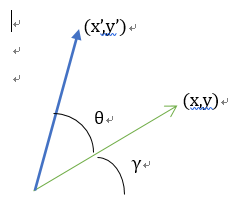
\includegraphics[width=3cm]{geometry/move.png}

\pause
\begin{displaymath}
|V|\cos(\theta + \gamma)=x' \ \ |V|\cos(\gamma)=x
\end{displaymath}

\begin{displaymath}
x'=\frac{ x \cos(\theta + \gamma) }{ \cos(\gamma) }=\frac{ x(\cos(\theta)\cos(\gamma) - \sin(\theta)\sin(\gamma) ) }{ \cos(\gamma) }
\end{displaymath}

\end{frame}

\begin{frame}

\pause
\begin{displaymath}
=x\cos(\theta)-x\sin(\theta)\tan(\gamma)=x\cos(\theta)-\sin(\theta)y
\end{displaymath}

\pause
同理可以求得$y'=x\sin(\theta)+y\cos(\theta)$

\pause
所以$rot((x,y),\theta)=(x\cos(\theta)-y\sin(\theta),x\sin(\theta)+y\cos(\theta))$

\pause
同时我们注意到向量的旋转是可以用矩阵乘法表示的
\begin{displaymath}
    [x \ y]*
    \left[
        \begin{array}{c @{\ } c}
            \cos(\theta)  & \sin(\theta) \\
            -\sin(\theta) & \cos(\theta)
        \end{array}
    \right]
\end{displaymath}
\end{frame}

\begin{frame}
\frametitle{向量的夹角}
求向量$\overrightarrow{a}$和向量$\overrightarrow{b}$的夹角

\begin{block}{方法一：}
$atan2(y_a,x_a)-atan2(y_b,x_b)$
\end{block}

\begin{block}{方法二：}
\begin{multicols}{2}
$atan2(\overrightarrow{a} \times \overrightarrow{b},\overrightarrow{a} \cdot \overrightarrow{b})$

解释：

$\overrightarrow{a} \times \overrightarrow{b}=|CD|*|AB|$

$\overrightarrow{a} \cdot \overrightarrow{b}=|AD| * |AB|$

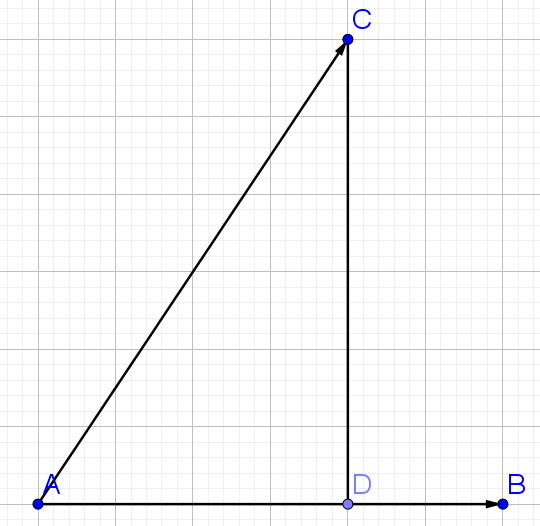
\includegraphics[height=2.5cm,width=3cm]{geometry/vector.png}
\end{multicols}
\end{block}

\pause
采用方法二更加好，因为方法一还要特判跨越了$\pi$到$-\pi$的情况，方法二不需要任何特判。
\end{frame}

\subsection{极角}

\begin{frame}
我们一般以x轴正方向为0刻度，从x轴正方向开始逆时针为正，顺时针为负。以x轴负方向为分界线。

特别地，x轴负方向的极角为$\pi$
\end{frame}

\subsection{重心}

\begin{frame}{三角形的重心}

三角形的重心是三条中线的交点。同时，重心把每条中线按照$1:2$的比例分割。

\pause
\begin{center}
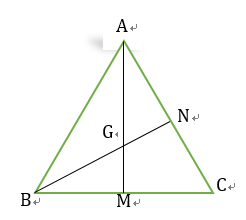
\includegraphics[width=3cm]{geometry/triangle.png}
\end{center}

\pause
\begin{displaymath}
M=\frac{B+C}{2}
\end{displaymath}
\begin{displaymath}
G=\frac{2}{3}M+\frac{1}{3}A=\frac{A+B+C}{3}
\end{displaymath}
\end{frame}

\begin{frame}{多边形的重心}

有一个定理：n个坐标为P，质量为M的质点的重心为

\begin{displaymath}
\sum_{i=1}^{n} P_i * \frac{M_i}{\sum_M}
\end{displaymath}

\pause
我们可以先把多边形进行三角剖分，然后得到所有三角形的重心，再以面积为权值计算加权平均数就是多边形的重心。
\end{frame}

\subsection{外心}
\begin{frame}

外心是指三角形外界圆的圆心

\pause
$\triangle ABC$解方程法

\begin{equation}
    (x-x_A)^2+(y-y_A)^2=(x-x_B)^2+(y-y_B)^2
\end{equation}
\begin{equation}
    (x-x_A)^2+(y-y_A)^2=(x-x_C)^2+(y-y_C)^2
\end{equation}

\pause
设
\begin{displaymath}
    A1=2(x_A-x_B),A2=2(x_A-x_C)
\end{displaymath}

\begin{displaymath}
    B1=2(y_A-y_B),B2=2(y_A-y_C)
\end{displaymath}

\begin{displaymath}
    C1=x_A^2+y_A^2-x_B^2-y_B^2,C2=x_A^2+y_A^2-x_C^2-y_C^2
\end{displaymath}
\end{frame}

\begin{frame}
\pause
\begin{equation}
    A1x+B1y=C1
\end{equation}
\begin{equation}
    A2x+B2y=C2
\end{equation}

\pause
根据克莱默法则
\begin{equation}
    x=\frac{ (C1*B2)-(C2*B1) }{ (A1*B2)-(A2*B1) }
\end{equation}
\begin{equation}
    y=\frac{ (A1*C2)-(A2*C1) }{ (A1*B2)-(A2*B1) }
\end{equation}
\end{frame}

\begin{frame}{几何法}

    也可以用几何法球外心

    外心就是三角形三条边垂直平分线的交点

    求出垂直平分线以后变成直线求交问题
\end{frame}

\subsection{内心}
\begin{frame}

三角形的内心为内切圆的圆心。\newline \newline

\href{https://en.wikipedia.org/wiki/Incenter}{\textcolor{purple}{维基}}上说三角形内切圆的圆心是三角形三个顶点A,B,C关于对边长度a,b,c的加权平均数，即
\begin{displaymath}
    inCenter=\frac{A*a+B*b+C*c}{a+b+c}
\end{displaymath}

（证明我不太懂，感兴趣的可以自行查阅）
\end{frame}

\section{直线、线段}

\subsection{直线的表示方法}
\begin{frame}
\frametitle{斜截式和两点/向量式}
\pause
直线的存储有多种方式。\newline \newline

\pause
一种是利用直线的斜截式方程y=kx+b。

这种表达方式方便判断直线的平行、求直线的交点、判断点与直线的位置关系都非常方便。但是它不能表示一条竖线，所以会受到很多的限制。\newline \newline

\pause
另一种是最常用的方法，直接存储直线上任意两个不同点的坐标$(a(x_1,y_1 ),b(x_2,y_2))$。

因为两点确定一条直线。同时，直线上的任意一个点都可以表示为$a+ \lambda (b-a)$的形式。
\end{frame}

\begin{frame}
\frametitle{一般式}
\pause
还有一种是直线的一般式$Ax+By+C=0$，它是唯一一个没有限制的直线方程，不需要考虑斜率为0、斜率为$\infty$等情况。

特别地，知道直线上两个不同的点$a,b$之后可以快速求得直线的一般式$A=y_b-y_a,B=x_b-x_a,C=x_ay_b-x_by_a$

\pause
通过直线的一般式$Ax+By+C=0$也可以快速得到直线上的两个点。

令$T=A^2+B^2$，则
\begin{displaymath}
x_1=-C*A/T,x_2=x_1+B
\end{displaymath}
\begin{displaymath}
y_1=-C*B/T,y_2=y_1-A
\end{displaymath}
\end{frame}

\subsection{直线求交}
\begin{frame}
\frametitle{向量法}
\pause
如果是两点式存储直线，那么就需要用到叉积来求交点。

\pause
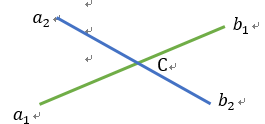
\includegraphics[width=3cm]{geometry/line.png}

\pause
$\Delta a_1 a_2 b_2$和$\Delta b_1 a_2 b_2$是同底三角形，面积之比就等于高之比。

根据平行线分线段成比例定理。这个比值也等于$|a_1 C|:|b_1 C|$

所以，我们可以得到C坐标的表达式。

\pause
\begin{displaymath}
a_1+(b_1-a_1)\frac{(S_{\Delta} a_1 a_2 b_2)}{(S_{\Delta} a_1 a_2 b_2+S_{\Delta} b_1 a_2 b_2)}
\end{displaymath}
\begin{displaymath}
=a_1+(b_1-a_1)\frac{(a_1-a_2)\times(b_2-a_2)}{(a_1-a_2 )\times(b_2-a_2 )+(b_2-a_2)\times(b_1-a_2)}
\end{displaymath}

\end{frame}

\begin{frame}
\frametitle{解析法}
\pause
如果用的是斜截式$y=k_1x+b_1,y=k_2x+b_2$(前提是斜率不为$\infty$)。

\pause
如果k,b都相同则无限交点

如果k相同b不相同则无交点

否则交点的横坐标为$-(b_1-b_2)/(k_1-k_2)$，再带入即可求出纵坐标

\pause
如果用的是一般式$A_1x+B_1y+C_1,A_2x+B_2y+C_2$

\pause
令$S=A_1B_2-A_2B_1,X=C_1B_2-C_2B_1,Y=A_1C_2-A_2C_1$

若$S=0$
	
\ \ \ \ 若$X=Y=0$，则无限交点

\ \ \ \ 否则无交点

否则$x_P=X/S,y_P=Y/S$
\end{frame}

\subsection{判点在线段上}
\begin{frame}
\pause
要判断点k是否在线段AB上，首先要判断k是否在直线AB上。

\pause
直接判$(k-A)$和$(B-A)$的叉积是否为0.

然后还要要求k位于AB之间，即$(A-k) \cdot (B-k) \le 0$
\end{frame}

\subsection{点到直线的投影}
\begin{frame}
\pause
现在要求T在直线AB上的投影

\pause
首先可以用点积求出投影离A的距离$d=\frac{ (B-A) \cdot (T-A) }{ |AB| }$

\pause
然后交点的位置即为$A+(B-A)*\frac{d}{|AB|}$

\pause
注意到点积计算的是有向距离，所以投影不在线段AB上的情况也没问题。
\end{frame}

\subsection{点到线段的最近点}
\begin{frame}
\pause
要求T到线段AB的最近点。分两种情况讨论。

\pause
如果T在直线AB上的投影在线段AB上\footnote{用点积快速判定}，则最近点为投影点。

\pause
否则最近点为A和B中的一个。
\end{frame}

\subsection{两条线段的最近距离}
\begin{frame}
\pause
如果两条线段AB和CD相交，那么距离为0。

否则距离为$\min(A$到$CD$距离，$B$到$CD$距离，$C$到$AB$距离，$D$到$AB$距离$)$ \newline \newline

\pause
证明可以分情况讨论

\pause
如果AB和CD是平行的，那么显然是正确的

\pause
否则我们考虑直线AB和直线CD的交点T。

\pause
如果T既在AB上又在CD上，则直接取T为答案，距离为0。

如果T只在AB上，那么我们会选择C和D中距离T最近的那一个。

如果T既不在AB上也不在CD上，则我们会取AB中距离T最近的一个和CD中距离T最近的那一个。
\end{frame}

\include{geometry/part3}
\section{半平面交}

\subsection{半平面的存储}
\begin{frame}
\pause
一条直线把平面划分成两个区域，其中的任意一个区域就叫做半平面。

\pause
半平面一般用带顺序的两点式直线来表示。对于直线(a,b)，我们默认它代表的半平面为向量ab沿逆时针方向扫描180$^{o}$经过的区域。
\end{frame}

\subsection{半平面交}
\begin{frame}
\pause
即给定若干个半平面，求出它们的公共部分。

\pause
求解半平面交的方法是：首先把所有表示半平面的直线向量进行极角排序，极角相同的把被包含的那个保留，其它的删除。

\pause
然后按照极角从小往大加入半平面。并用一个deque维护当前已经加入的半平面。加入一个半平面时，如果队列尾部和尾部前一个元素的交点不在当前半平面内，则弹出队列尾。同时也检查队首，如果队列首部和首部下一个元素不在当前半平面内也将其删除。

\pause
在加入完所有的半平面后，还要做一次队列首尾交接的工作。如果队列首部和首部的下一个元素不在队尾的半平面内则把队首弹出。如果队列尾部和尾部的前一个元素不在队首的半平面内则把队尾弹出
\end{frame}
\section{多边形与圆}

\subsection{多边形的面积}
\begin{frame}
\pause
三角形的面积可以用叉积快速求，多边形的面积可以以某个点为中心，把多边形分成若干个三角形，然后对所有三角形面积求和相加。

\pause
同时，叉积计算的是有向面积，所以中心也可以在多边形之外。

\pause
一般我们选取中心为原点$(0,0)$，这样可以避免向量减法，减小常数。
\end{frame}

\subsection{点在多边形内的判定}
\begin{frame}
\pause
点在多边形内的判定一般用射线法。

\pause
从询问点随机一个角度射出一条射线，如果射线与奇数条多边形的边相交则在多边形内，否则不在。

\pause
需要注意的是如果射线正好设在了某两条线段的交点上则不方便处理，重新随机一条射线就可以了。
\end{frame}

\subsection{圆和直线的交点}
\begin{frame}
\frametitle{求圆$(x,y,R)$和直线$AB$的交点}

\pause
方法一：直接解方程求出交点坐标。

\pause
方法二：首先求出圆心到直线的距离dis。如果$dis>R$则显然无交点。

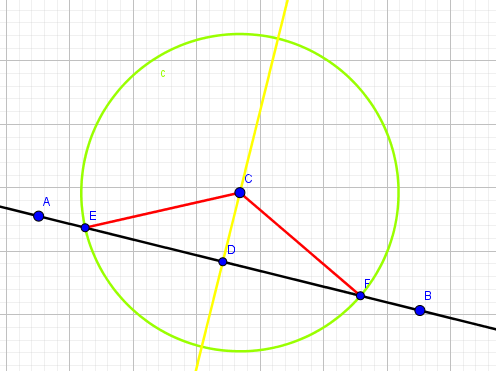
\includegraphics[width=4cm]{geometry/circle.png}

作出C到AB的垂足D。那么$\angle ECD=\angle FCD=acos(dis/R)$。

这样我们就可以得到CE和CF的极角。然后就可以计算出E和F的坐标。
\end{frame}

\subsection{圆和圆的交点}
\begin{frame}
\frametitle{求圆$(x_1,y_1,R_1)$和圆$(x_2,y_2,R_2)$的交点}

\pause
方法一：最直接的方法：解方程。

\pause
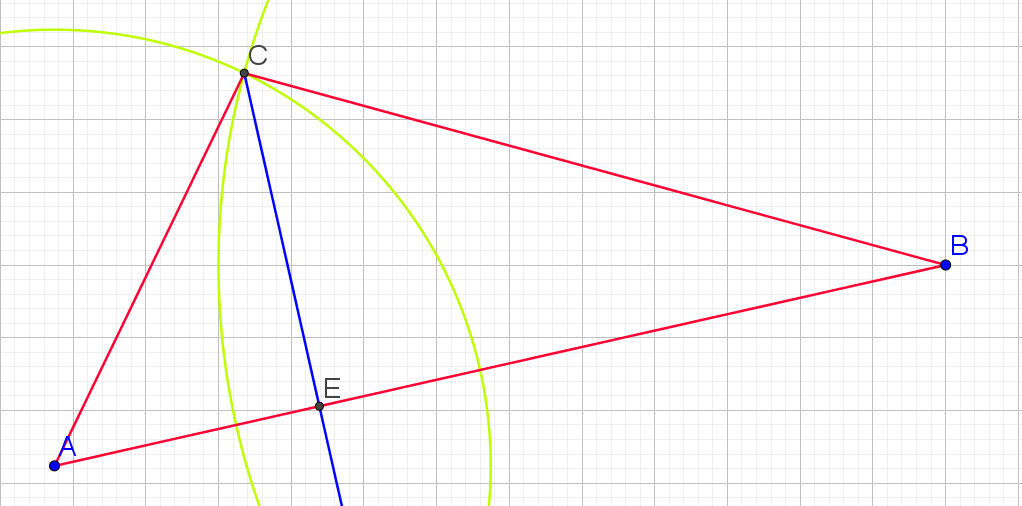
\includegraphics[width=6cm]{geometry/circle2.png}

方法二：我们已知$|AC|=R_A,|BC|=R_B,|AB|$，可以用海伦公式求出$\Delta ABC$的面积，然后得到$CE$

这样也可以知道$|AE|$，就能求出E的坐标，然后再求出点C

\pause
方法三：现在知道了$\overrightarrow{AB}$的极角，可以用余弦定理求出$\angle CAB$，那么就知道了$\overrightarrow{AC}$的极角，直接得到C的坐标。

一般采用方法三，方法二要特判E在线段AB的延长线上的情况。
\end{frame}

\subsection{点和圆的切线}
\begin{frame}
\frametitle{求点B到圆A的切线}
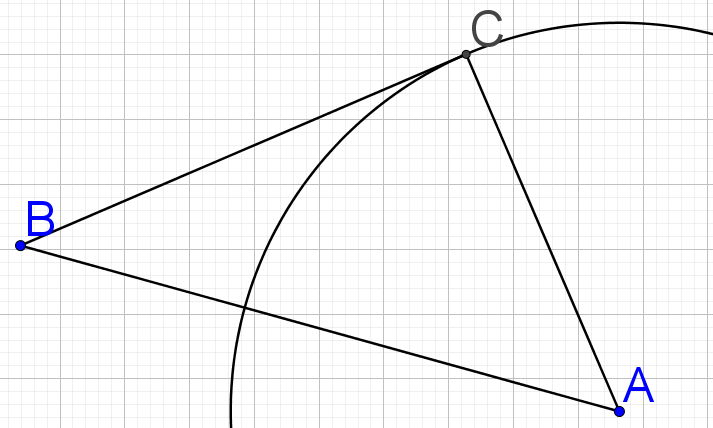
\includegraphics[height=5cm]{geometry/circle3.png}

\pause
利用反三角函数求出$\angle CBA$，然后得到$\overrightarrow{BC}$的极角，从而得到C的坐标
\end{frame}

\subsection{圆与圆公切线}
\begin{frame}
\frametitle{求圆A和圆B的公切线}
\pause
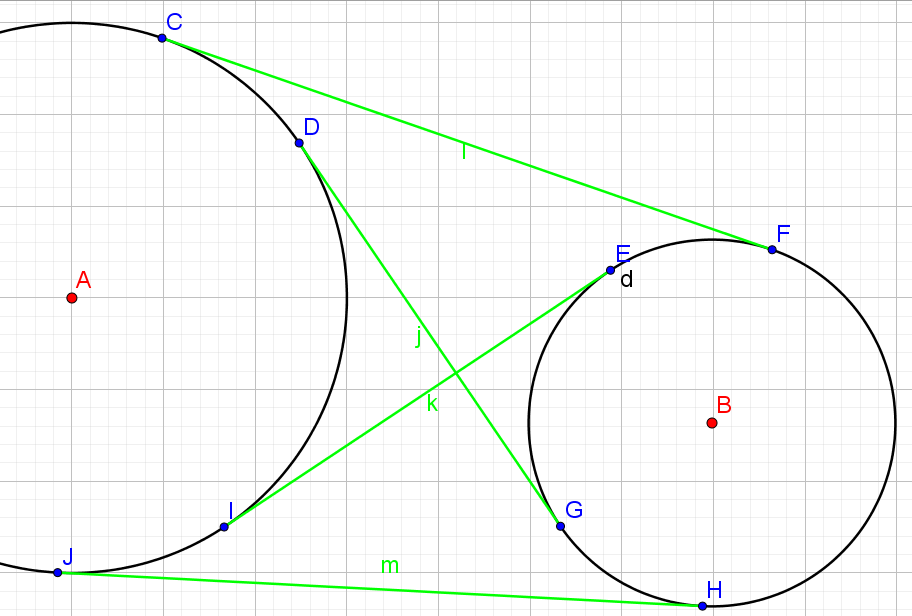
\includegraphics[height=5cm]{geometry/circle4.png}

圆与圆有4条公切线，分别为两条内公切线和两条外公切线
\end{frame}

\begin{frame}
\frametitle{求圆A和圆B的公切线}
\framesubtitle{Case1:内公切线}
\pause
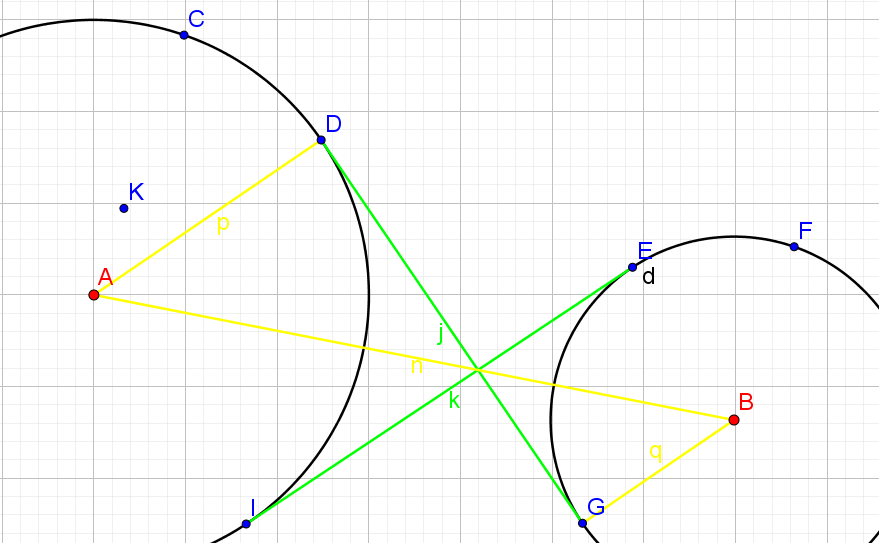
\includegraphics[height=4cm]{geometry/circle5.png}

可以先求出$\angle DAB$，然后求出点D
\begin{displaymath}
    \angle DAB=acos\left( \frac{R_A}{ |AB| * \frac{R_A}{R_A+R_B} } \right)=acos\left( \frac{R_A+R_B}{|AB|} \right)
\end{displaymath}
\end{frame}

\begin{frame}
\frametitle{求圆A和圆B的公切线}
\framesubtitle{Case2:外公切线}
\pause
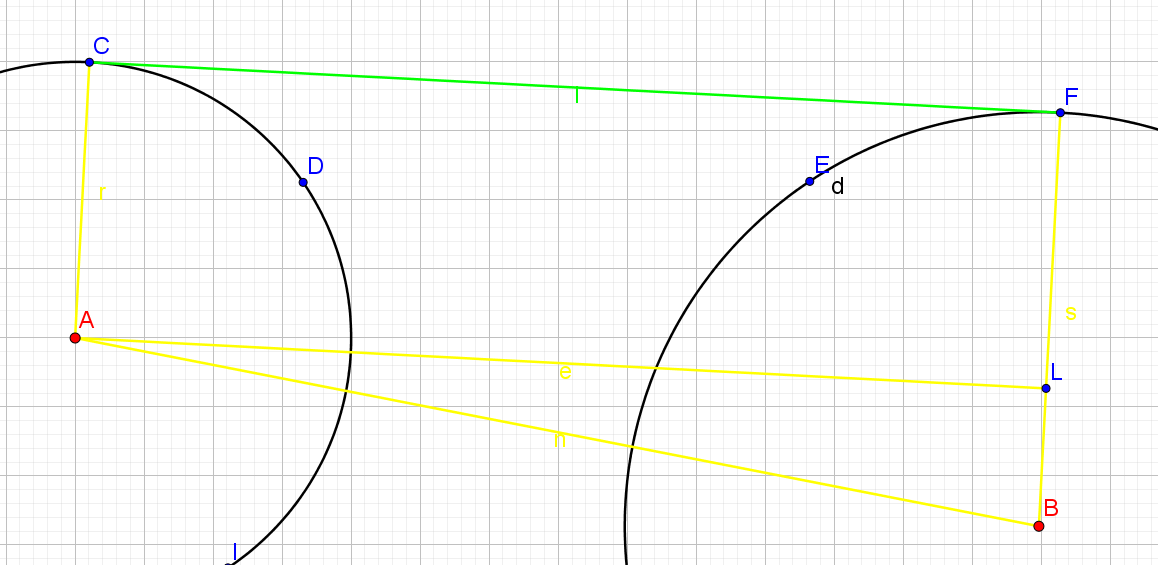
\includegraphics[height=4cm]{geometry/circle6.png}

可以先求出$\angle CAB$，然后求出点C
\begin{displaymath}
    \angle CAB=asin\left( \frac{R_B-R_A}{|AB|} \right)+\frac{\pi}{2}
\end{displaymath}
同时注意到sin是可以为负数的，所以也可以处理$R_B<R_A$的情况
\end{frame}


\part{2}
\begin{frame}{Part2}{难点}
\begin{multicols}{2}
\tableofcontents
\end{multicols}
\end{frame}

\include{geometry/part6}
\section{反演}

\begin{frame}
\pause
反演是一种几何变换。

给定点$O$、常数$k$，点$P$的变换对应点就是在以O开始的射线OP上的一点$P'$使得$|OP||OP'|=k^2$。 \newline \newline
\pause
点$\rightarrow$点

过O的直线$\rightarrow$过O的直线；不过O的直线$\rightarrow$过O的圆

过O的圆$\rightarrow$不过O的直线；不过O的圆$\rightarrow$不过O的圆

过O的球$\rightarrow$不过O的平面 \newline \newline
\pause
对于两个不在反演中心的点$A,B$，它们的反演对应点为$A',B'$，那么$|A'B'|=\frac{k}{|OA|*|OB|}|AB|$。

\end{frame}
\section{平面图}

\subsection{基本定义}

\begin{frame}{平面图定义}
若图G可画在平面上，使得任意两条边都不会在非端点处相交，则称G是平面图。
\end{frame}

\subsection{欧拉定理}
\begin{frame}{欧拉定理}
欧拉定理建立了平面图中点数、边数和域数的关系，可以知二求一。 \newline \newline

对于平面图，如果有F个面，E条边，V个点，k个连通块，那么有公式

$F=E-V+k+1$

证明：使用归纳法。当$E=0$时，$k=V$，等式成立。然后一条一条加边，如果加入边的两个点未联通，则$k--,E++$，等式不变。如果加入的两个点已联通，则这条边必然把某个域一分为二，等式两边同时$+1$，得证。
\end{frame}

\begin{frame}{性质}
\begin{itemize}
    \item $E \le 3n-6$
        \begin{proof}
            每个域至少有三条边，每条边最多与两个域相连，所以$F \le \frac{2}{3}E$

            那么$E-V+k+1 \le \frac{2}{3}E$，同时有$k \ge 1$，所以$E \le 3n-6$
        \end{proof}
    \item $k \le 2n-4$
        \begin{proof}
            把$F \le \frac{2}{3}E$的E用欧拉公式代换得

            $\frac{3}{2}F \le F+V-k-1 \rightarrow F \le 2V-2k-2$,同时有$k \ge 1$,得证
        \end{proof}
\end{itemize}
\end{frame}

\begin{frame}{P3776 [APIO2017] 斑斓之地}
    题目描述：一个 $r \times c$ 的方格表，一只蛇在上面爬导致部分方格表变成了河。多次询问，每次询问只保留某个矩形内的格子，问非河的部分形成了多少个连通块。
\end{frame}

\begin{frame}{P7295 [USACO21JAN] Paint by Letters P}
    考虑这样一个问题：给你一棵树，只考虑区间 \([l,r]\) 中的点，形成几个连通块（数量只需要求为 \(\leq i < j \leq r\) 且 \((i,j) \in E\) 的 \((i,j)\) 数量（可以认为是边点之类的东西）。

    一般平面图也可以套用这个做法。本题中在相邻非网格子之间连边，那么只需要反映：点数、面数和边数。

    点数容易，那么真难则反扫描线以下即可（如果强制在线，就主席树），边数几乎一样。

    考虑可能出现什么样的“面”。首先所有 \(2 \times 2\) 的矩形一定是他的，还有没有其他的？

    蛇的形态非常关键——所有河都是连通的。因此，还有另一种环——包裹了整条蛇的环，单独处理一下就行。
\end{frame}


\subsection{平面图与对偶图}

\begin{frame}{平面图对偶图定义}

\begin{multicols}{2}
    
对偶图：

原图的每个域成为新图的一个点

原图的每个点作为新图的一个域

\begin{center}
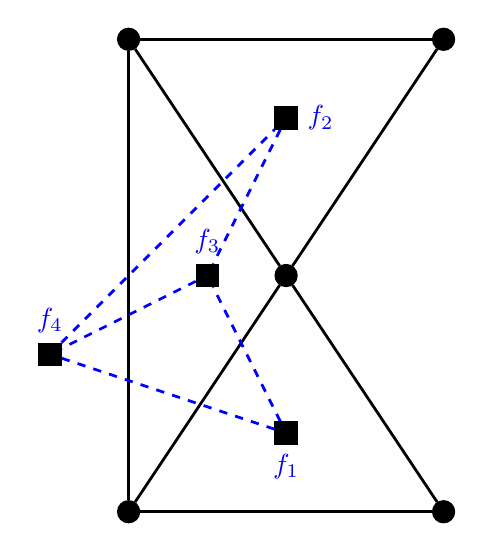
\begin{tikzpicture}[
    node distance=1.5cm,
    vertex/.style={circle, minimum size=8pt, draw, fill=black, inner sep=0pt},
    dual_vertex/.style={rectangle, draw, fill=black, minimum size=8pt, inner sep=0pt},
    edge/.style={line width=1pt},
    dual_edge/.style={line width=1pt, blue, dashed}
]

% 绘制平面图节点
\node[vertex] (v1) at (0,0) {};
\node[vertex] (v2) at (4,0) {};
\node[vertex] (v3) at (2,3) {};
\node[vertex] (v4) at (0,6) {};
\node[vertex] (v5) at (4,6) {};

% 绘制平面图边
\draw[edge] (v1) -- (v2);
\draw[edge] (v1) -- (v3);
\draw[edge] (v2) -- (v3);
\draw[edge] (v3) -- (v4);
\draw[edge] (v3) -- (v5);
\draw[edge] (v4) -- (v5);
\draw[edge] (v1) -- (v4);

% 绘制对偶图节点（面）
\node[dual_vertex] (f1) at (2,1) {};
\node[dual_vertex] (f2) at (2,5) {};
\node[dual_vertex] (f3) at (1,3) {};
\node[dual_vertex] (f4) at (-1,2) {};

% 绘制对偶图边
\draw[dual_edge] (f4) -- (f2);
\draw[dual_edge] (f1) -- (f3);
\draw[dual_edge] (f1) -- (f4);
\draw[dual_edge] (f2) -- (f3);
\draw[dual_edge] (f3) -- (f4);

% 标记对偶图节点
\node[blue, below] at (f1.south) {$f_1$};
\node[blue, right] at (f2.east) {$f_2$};
\node[blue, above] at (f3.north) {$f_3$};
\node[blue, above] at (f4.north) {$f_4$};

\end{tikzpicture}
\end{center}
\end{multicols}

\end{frame}

\begin{frame}{平面图转对偶图}{算法}
将每条边拆分成两条有向边，并将每个点出发的有向边按顺时针排序。

选择任意一条未访问的边出发，在每个节点处选择绕该点顺时针旋转遇到的第一条边为下一条边，直到回到初始边。这样就走完的一个域周围的边。不断重复，直到所有边均被走过。

为每个域建立一个点。如果一条无向边被两个域共用，那么在这两个域之间连上这条边
\end{frame}

\begin{frame}
\frametitle{对偶图的应用}
\begin{multicols}{2}
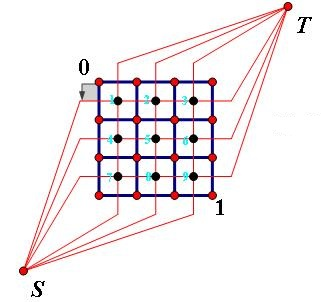
\includegraphics[width=5cm]{geometry/duioutu.jpg}

\begin{center}
平面图最大流
\begin{displaymath}
    \Downarrow
\end{displaymath}

平面图最小割
\begin{displaymath}
    \Downarrow
\end{displaymath}
对偶图最短路
\end{center}
\end{multicols}
\end{frame}

\begin{frame}{P4001 ICPC-Beijing 2006 狼抓兔子}

\begin{minipage}{0.4\textwidth}
    
给定这样一张网格图：左上角点为 $(1,1)$，右下角点为 $(N,M)$（图中 $N=3$，$M=4$）。有以下三种类型的道路：

1. $(x,y)\rightleftharpoons(x+1,y)$

2. $(x,y)\rightleftharpoons(x,y+1)$

3. $(x,y)\rightleftharpoons(x+1,y+1)$
\end{minipage}
\hfill % 两列之间的间距
\begin{minipage}{0.58\textwidth}
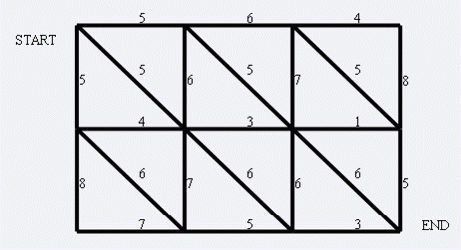
\includegraphics[width=\textwidth]{geometry/planar.png}
\end{minipage}


道路上的权值表示这条路上最多能够通过的兔子数，道路是无向的。左上角和右下角为兔子的两个窝，开始时所有的兔子都聚集在左上角 $(1,1)$ 的窝里，现在它们要跑到右下角 $(N,M)$ 的窝中去，狼王开始伏击这些兔子。当然为了保险起见，如果一条道路上最多通过的兔子数为 $K$，狼王需要安排同样数量的 $K$ 只狼，才能完全封锁这条道路，你需要帮助狼王安排一个伏击方案，使得在将兔子一网打尽的前提下，参与的狼的数量要最小。($N,M \le 1000$)
\end{frame}

\begin{frame}{P2046 [NOI2010] 海拔}
    YT 市是一个规划良好的城市，城市被东西向和南北向的主干道划分为 $n \times n$ 个区域。简单起见，可以将 YT 市看作 一个正方形，每一个区域也可看作一个正方形。从而，YT 城市中包括 $(n+1) \times (n+1)$ 个交叉路口和 $2n \times (n+1)$ 条双向道路（简称道路），每条双向道路连接主干道上两个相邻的交叉路口。下图为一张 YT 市的地图（$n = 2$），城市被划分为 $2 \times 2$ 个区域，包括 $3 \times 3$ 个交叉路口和 $12$ 条双向道路。

    小 Z 作为该市的市长，他根据统计信息得到了每天上班高峰期间 YT 市每条道路两个方向的人流量，即在高峰期间沿着该方向通过这条道路的人数。每一个交叉路口都有不同的海拔高度值，YT 市市民认为爬坡是一件非常累的事情，每向上爬 $h$ 的高度，就需要消耗 $h$ 的体力。如果是下坡的话，则不需要耗费体力。因此如果一段道路的终点海拔减去起点海拔的值为 $h$（注意 $h$ 可能是负数），那么一个人经过这段路所消耗的体力是 $\max\{0, h\}$。

    小 Z 还测量得到这个城市西北角的交叉路口海拔为 $0$，东南角的交叉路口海拔为 $1$（如上图所示），但其它交叉路口的海拔高度都无法得知。小 Z 想知道在最理想的情况下（即你可以任意假设其他路口的海拔高度），每天上班高峰期间所有人爬坡消耗的总体力和的最小值。
\end{frame}

\begin{frame}{P10665 [AMPPZ2013] Bytehattan}
\end{frame}

\begin{frame}{P4646 [IOI 2007] flood 洪水}
\end{frame}

\begin{frame}{P7916 [CSP-S 2021] 交通规划}
\end{frame}

\begin{frame}{CF750H. New Year and Snowy Grid}
    有一张有障碍的$h \times w$的网格图，问是否存在一条路径，从左上角出发到右下角，再回到左上角，且不会重复经过同一个点（起点除外）。
    
    有$q$组询问，每组询问给出$k$个非障碍点，问是否存在不经过这$k$个点的合法路径。

    $h,w \le 10^3，q \le 10^4，k \le 10$
\end{frame}

\begin{frame}{CF750H. New Year and Snowy Grid}
    \begin{itemize}
        \item 首先，问题相当于求起点到终点是否存在两条不相交的路径。
        \item 如果只有一组询问的话，那就是一个经典的网络流模型，我们可以给每个点拆点，如果这个点是障碍点，那么$i$向$i'$连流量为$0$的边，否则，$i$向$i'$连流量为$1$的边，表示每个点只能经过一次。再每个点向其周围的$4$个点连流量为$1$的边。
        \item 然后从$S$到$T$跑一边最大流，如果流量小于$2$，那么答案就是NO，否则就是YES。
        \item 接着我们可以把最大流问题转换成最小割问题，不过遗憾的是之前的建图并不是平面图，不能转换成最短路问题。
    \end{itemize}
\end{frame}

\begin{frame}{CF750H. New Year and Snowy Grid}
    \begin{itemize}
        \item 我们可以用一个巧妙的办法，直接考虑最短路模型，S向所有$(i,1)(2 \le i \le n)$和$(n,j)(1 \le j<m)$连边，也就是最左边的那一列和最下边的那一行。所有$(i,m)(1 \le i<n)$和$(1,j)(2 \le j \le m)$向$T$连边，也就是最右边的那一列和最上边的那一行。
        \item 然后所有点向八联通方向连边，边没有边权，每个点有点权，障碍点的点权为0，空地的点权为1。
        \item 跑一遍最短路，如果最短路小于$2$，那么答案就是NO，否则就是YES。
        \item 这样的复杂度就是最短路的复杂度了，考虑到点权只有$0$和$1$，我们可以bfs，于是，做一遍复杂度与图的边数有关，即$O(8nm)$的。
    \end{itemize}
\end{frame}

\begin{frame}{CF750H. New Year and Snowy Grid}
    \begin{itemize}
        \item 当然，继续观察可以发现，由于只要判断最短路与2的大小关系，所以问题就转化成：是否添加一个障碍物就可以使S到T的最短路为0，也就是，是否可以添加一个障碍物使得$S$和$T$联通。
        \item 关于联通性，很容易想到用并查集维护。
        \item 于是我们可以预处理出所有的障碍物形成的连通块，并预处理出所有相距为1的连通块对。
        \item 每次询问，把$k$个点周围的点用并查集连起来，最后看一下，所有与S并起来的连通块和所有与T并起来的连通块，是否存在连通块对相距为1，以及是否有新添的障碍点，满足这个点到S集的距离加上这个点到T集的距离不超过1。
    \end{itemize}
\end{frame}

\begin{frame}{平面图点定位}
\begin{multicols}{2}
平面图点定位求的是对于平面图中的一个点，它位于对偶图中的哪个域。

直接求解二维问题比较麻烦，我们的简化方法是把它进行梯形剖分。

基本假设：所有点横坐标互异(可以把所有点的x坐标随机扰动eps范围，保证没有相同横坐标)

在这个结构中，每个域均是梯形(三角形可看做是退化的梯形)。且域数仍然为O(n) \newline \newline

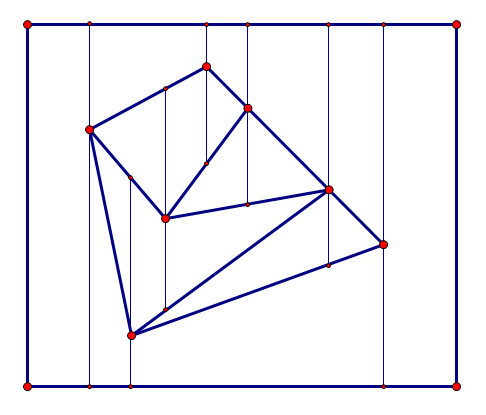
\includegraphics[width=5cm]{geometry/place.png}
\end{multicols}
\end{frame}
\begin{frame}
\frametitle{平面图点定位}
\begin{proof}
证明：每个点引出两条射线，至多增加两个节点。故节点总数不超过3*n。除节点处无交点，仍然是平面图。故域的数量仍是O(n)。
\end{proof}

如何构建这样一张平面图呢？我们用扫描线来完成。

把所有x坐标离散化，那么$x_{i-1} \ldots x_i$这段区间内的域和$x_i \ldots x_{i+1}$这段域的区别就在于有一些域在$x_i$结尾，应当删除，有一些域在$x_i$开头，应当加入。

然后注意到，$x_i \ldots x_{i+1}$这段区间内的所有域在纵坐标上是有严格的大小关系的，我们可以按照大小关系存储这些域。这样查询一个点的位置只需要二分就可以了。需要支持删除与插入，可以用一棵平衡树来实现。

如果需要在线，可以把平衡树可持久化。
\end{frame}

\begin{frame}{P4073 [WC2013] 平面图}
\end{frame}

\begin{frame}{P3249 [HNOI2016] 矿区}
\end{frame}


\subsection{三角剖分与V图}

\begin{frame}{Delaunay三角剖分}

假设V是二维实数域上的有限点集，边e是由点集中的点作为端点构成的封闭线段，E为e的集合。那么该点集V的一个三角剖分T=(V,E)是一个平面图G。

该平面图满足条件：
\begin{enumerate}
    \item 除了端点，平面图中的边不包含点集中的任何点。
    \item 没有相交边。
\end{enumerate}

平面图中所有的面都是三角面，且所有三角面的合集是点集V的凸包。
\end{frame}

\begin{frame}
\frametitle{Delaunay三角剖分}

Delaunay三角剖分是一种特殊的三角剖分。\newline \newline

Delaunay边：假设E中的一条边e(两个端点为A,B),e若满足下列条件，则称之为Delaunay边：存在一个圆经过A,B两点，圆内(注意是圆内，圆上最多三点共圆)不含点集V中任何其他的点，这一特性又称空圆特性。
\newline \newline

Delaunay三角剖分：如果点集V的一个三角剖分T只包含Delaunay边，那么该三角剖分称为Delaunay三角剖分。
\end{frame}

\begin{frame}{分治法构造Delaunay三角剖分}

首先对点集按x坐标排序。如果点集内点的个数小于等于3，那么直接构造，否则将点集拆分成两个大小差不多的点集进行构造，最后合并两点集的Delaunay三角剖分。\newline \newline

接下来考虑如何合并。
\end{frame}

\begin{frame}{分治法构造Delaunay三角剖分}{步骤一}
首先，求解两个点集的凸包的最下方的正切线,并连接两端点。

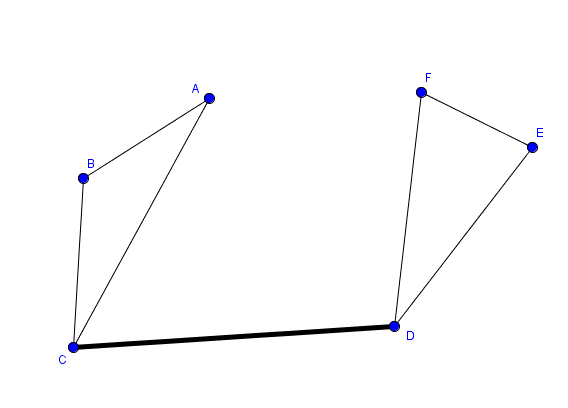
\includegraphics[height=5cm]{geometry/v1.png}
\end{frame}

\begin{frame}{分治法构造Delaunay三角剖分}{步骤二}
接下来，如图所示，CD为两个凸包的正切线，求出它们的中垂线$L_{CD}$。

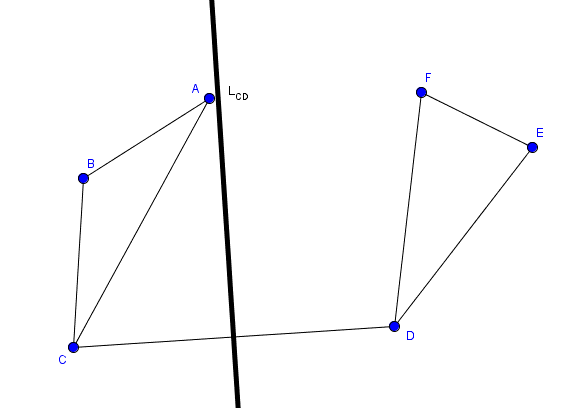
\includegraphics[height=5cm]{geometry/v2.png}
\end{frame}

\begin{frame}{分治法构造Delaunay三角剖分}{步骤三}
然后找到与C或D相连的边中，中垂线与$L_{CD}$有交点的边，如果有多个边，那么选择交点Y坐标最小的点所关联边。

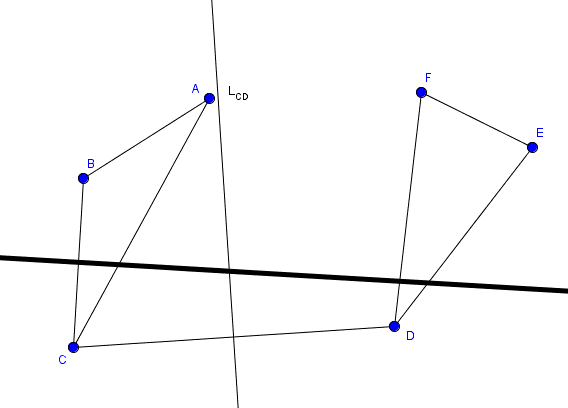
\includegraphics[height=5cm]{geometry/v3.png}
\end{frame}

\begin{frame}{分治法构造Delaunay三角剖分}{步骤四}
如图所示，选择的边为BC，那么连接BD，并且删除与BD相交的边。设BD为新产生的正切线。

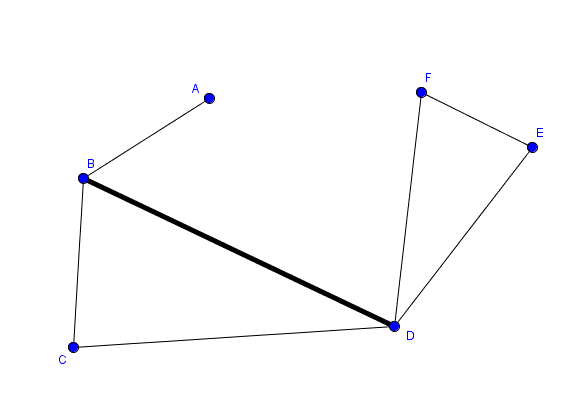
\includegraphics[height=5cm]{geometry/v4.png}
\end{frame}

\begin{frame}{分治法构造Delaunay三角剖分}{步骤五}
然后将BD像CD一样不断重复以上步骤，就可以合并两个点集的Delaunay三角剖分了。

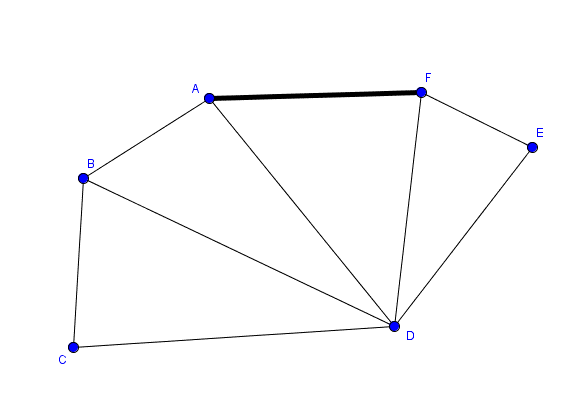
\includegraphics[height=5cm]{geometry/v5.png}
\end{frame}

\begin{frame}{分治法构造Delaunay三角剖分}{解释}

之前为什么选择交点纵坐标最小的边呢？

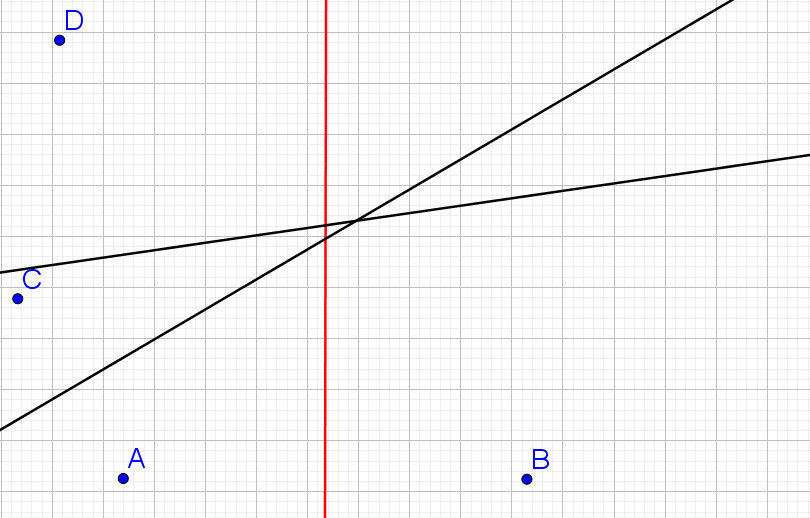
\includegraphics[height=2.5cm]{geometry/vgraph2.png}

考虑之前AC和AD都有边，AC的中垂线和AB的中垂线的交点在AD的中垂线和AB的中垂线的交点的下方。有一个结论：三个点两两的中垂线会相交于同一点，所以BC中垂线与AB的交点也会在BD中垂线与AB交点的下方。那
么BD中垂线就会被BC中垂线和BA中垂线完全覆盖，所以BD不能相邻。

把BC相连之后，如果存在D有AD与BC相交则AD的中垂线会被AC中垂线和AB中垂线覆盖，所以AD不能相邻。
\end{frame}

\begin{frame}{分治法构造Delaunay三角剖分}{优化}

分治法构建三角剖分的复杂度是期望nlogn的，但是可以被卡到平方以上。瓶颈在于上述操作3中，每次我们要访问A的所有出边和B的所有出边，找到中垂线交点纵坐标最小的边。但是操作结束之后只会有一个点进行改变，也就是说另外一个点可能会被访问多次。

这种情况也是很好hack的，在左侧构n/2个中垂线交点纵坐标很小的点，在右边构n/2个点与点B相连。那么每次都会访问一遍B，但是移动的变量永远是A。这样复杂度就达到了平方级别。

如何优化查找过程呢？
\end{frame}

\begin{frame}{分治法构造Delaunay三角剖分}{优化}
    
\begin{multicols}{2}
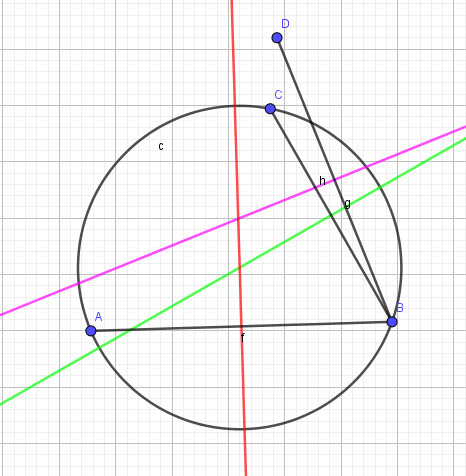
\includegraphics[width=5cm,height=5cm]{geometry/De.png} \newline \newline

现在B有两个备选出边BC和BD。其中$\angle ABC < \angle ABD$

如果D在ABC外接圆内,则BC边需要被立即删除。如果不在,则我们当前只需要考虑C点，而不需要考虑D点。

所以,只要维护一个点的所有出边的极角序,就可以快速查找。

现在我们需要支持的操作是：查询相邻点、插入、删除,把原本存边的邻接表改成双向链表就可以$O(1)$进行操作了。
\end{multicols}
\end{frame}

\begin{frame}{V图的定义}
定义$H(P_1,P_2)$为到$P_1$点比到$P_2$点距离近的点的集合。

对于平面上n个点的点集S,定义$V(P_i)=\bigcap_{i \neq j}H(P_i,P_j)$,即$V(P_i)$表示到$P_i$点的距离小于其他所有点的距离的点的集合,这显然是一个不多于$n-1$条边的凸多边形区域(有可能不闭合),称为关联与 $P_i$的Voronoi多边形或关联与$p_i$的Voronoi多边形域。

对于点集S中的每个点都可以做一个Voronoi多边形(域),这样n个Voronoi多边形(域)组成的图形叫做Voronoi图。
\end{frame}

\begin{frame}{V图的构造}
暴力构造法：对于每个点，求出所有的$H(P_i,P_j)$，然后对于$n-1$个半平面求交。$O(nlogn)$

Voronoi图与Delaunay三角剖分互为对偶图，所以可以先求出点集的Delaunay三角剖分，然后将图形对偶，这样就得到了Voronoi图。

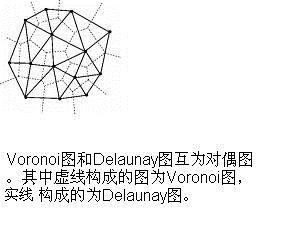
\includegraphics[height=5cm]{geometry/v.png}
\end{frame}

\begin{frame}{V图的构造}{对偶性证明}
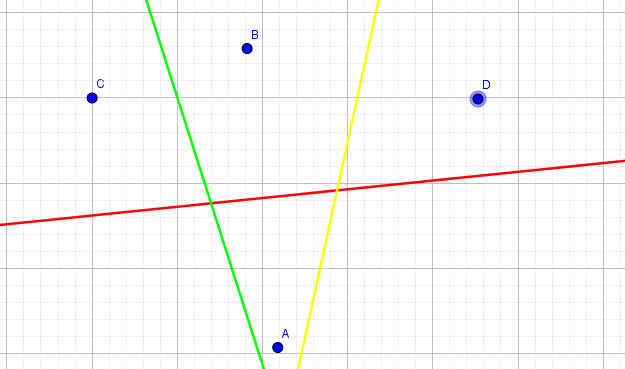
\includegraphics[height=4cm]{geometry/vgraph.png}

证明：在图中作出AB两个点的中垂线PQ，那么包含AB的圆一定在直线PQ上。
又由于圆P中不能包含其它点，对于任意点C满足P位于BC的中垂线的靠B一侧。

如果AB相连那么取红色直线中间夹的这一部分都是合法圆心。

如果AB不相连那么也不存在圆P。
\end{frame}

\begin{frame}
\frametitle{Delaunay三角剖分对偶得Voronoi图}
因为Voronoi点正好是三条Voronoi边的交点，也就是说Voronoi点是形成三边的三点的外接圆圆心。
那么对偶的方法就是：
\begin{enumerate}
    \item 先将每个Delaunay三角形的外接圆圆心求出。
    \item 如果两个三角形有公共边，那么在它们的外接圆圆心之间连一条边。
    \item 如果某一条Delaunay边在点集的凸包上，那么以这条边所在的三角形的外接圆圆心为起点，向该边做垂直射线。
\end{enumerate}

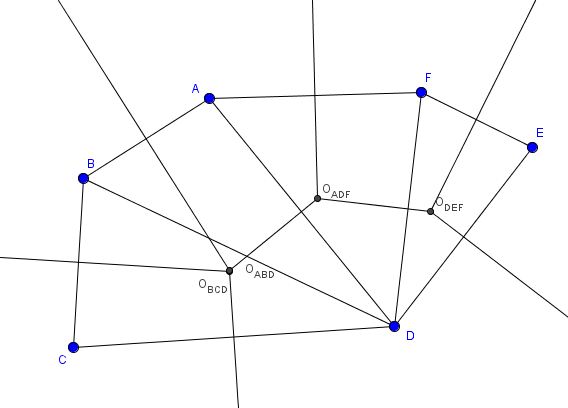
\includegraphics[height=3cm]{geometry/d.png}
\end{frame}

\begin{frame}
\frametitle{V图的应用}
\framesubtitle{平面MST问题}
\pause
给定平面上的一些点，要选择一些点对两两连边，两点之间的边长为欧几里得距离，求最小生成树。

\pause
结论：最小生成树上的边一定是Delaunay三角剖分中的边。

\pause
证明：根据Delaunay三角剖分的定义，如果ab之间没有边相连，则以ab为直径的圆中必然有其它点c。

而我们知道，圆内最大距离$=$直径，而ab就是直径，所以$|ac|,|bc| \le |ab|$

我们把边$(a,b)$删除，如果c在连通块a，则连接边$(c,b)$，否则连接边$(c,a)$，这样不会更差。

\pause
所以，构出三角剖分做最小生成树即可。复杂度$n(logn+\alpha(n))$
\end{frame}

\begin{frame}
\frametitle{V图的应用}
\pause
有一个$n*m$的矩形，矩形内有若干个点组成点集S。现在要把一个圆从矩形的左边平移到矩形的右边。要求圆不能和S中的点以及矩形边界相交。问圆的半径最大值。

\pause
问题实际上就是，找到一条路径，使得这条路径上的点到矩形边界和S中的点的最小距离最大。

\pause
经过分析可以发现，最优路线一定是沿V图中的边走。(如果偏离了V图中的边那么会使得到某个点的距离变小)

\pause
还要注意一个细节：可能是沿着边界走，所以我们对于所有点$(x,y)$都新建两个点$(x,0)$和$(x,m)$。

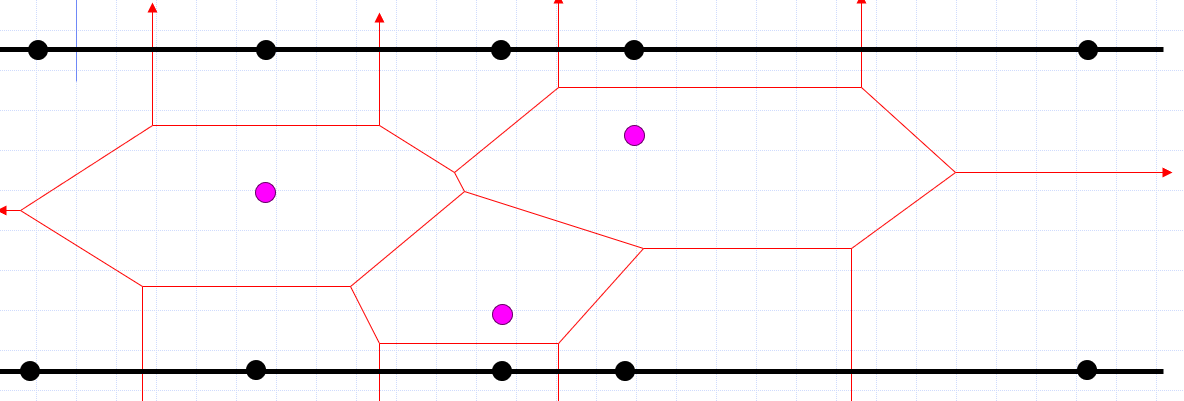
\includegraphics[height=2cm]{geometry/vgraph3.png}
\end{frame}


\part{3}
\begin{frame}
\frametitle{Part3}{三维计算几何}
\begin{multicols}{3}
\tableofcontents
\end{multicols}
\end{frame}

\section{基本定义}

\subsection{左右手系}
\begin{frame}
\pause
(x,y,z)满足右手系的定义为伸出右手，将四指由x轴指向沿小于平角的叫转到y轴指向，拇指所指的方向为z轴方向。

左手系也可类似定义。

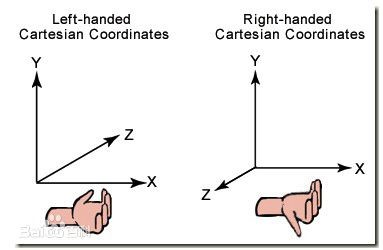
\includegraphics[height=3cm]{geometry/hand.png}

\end{frame}

\subsection{三维叉积}
\begin{frame}
\pause
三维叉积的计算是通过计算行列式$\left| \begin{array}{c @{\ } c @{\ } c} i & j & k \\ x_1 & y_1 & z_1 \\ x_2 & y_2 & z_2 \end{array} \right|$来得到的。

\pause
需要注意的是三维向量的叉积得到的还是一个向量$(y_1 z_2-y_2 z_1,x_2 z_1-x_1 z_2,x_1 y_2-x_2 y_1)$。

它的模长等于原来两个向量所围成的平行四边形的面积。
\end{frame}

\subsection{混合积}
\begin{frame}
\pause
$(\overrightarrow{a} \times \overrightarrow{b}) \cdot \overrightarrow{c}$ 为向量$\overrightarrow{a},\overrightarrow{b},\overrightarrow{c}$的混合积，它的含义是向量$\overrightarrow{a},\overrightarrow{b},\overrightarrow{c}$ 所围成的平行六面体的体积。
\end{frame}

\subsection{三维向量旋转}
\begin{frame}
\pause
三维空间中的旋转变换比二维空间中的旋转变换复杂。除了需要指定旋转角外，还需指定旋转轴。

若以坐标系的三个坐标轴x,y,z分别作为旋转轴，则点实际上只在垂直坐标轴的平面上作二维旋转。此时用二维旋转公式就可以直接推出三维旋转变换矩阵。

规定在右手坐标系中，物体旋转的正方向是右手螺旋方向，即从该轴正半轴向原点看是逆时针方向。
\end{frame}

\begin{frame}
\frametitle{绕坐标轴旋转}
\pause
\begin{multicols}{2}
Case \ 1:绕z轴旋转

$x'=x\cos(\gamma)-y\sin(\gamma)$

$y'=x\sin(\gamma)+y\cos(\gamma)$

$z'=z$

Case \ 2:绕x轴旋转

$y'=y\cos(\gamma)-z\sin(\gamma)$

$z'=y\sin(\gamma)+z\cos(\gamma)$

$x'=x$

Case \ 3:绕y轴旋转

$z'=z\cos(\gamma)-x\sin(\gamma)$

$x'=z\sin(\gamma)+\cos(\gamma)$

$y'=y$

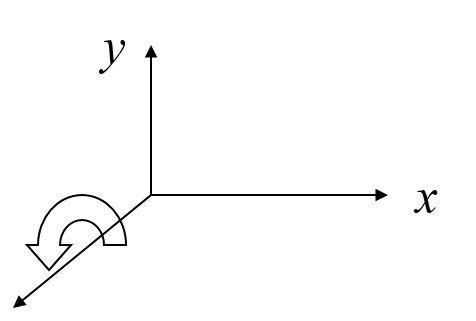
\includegraphics[height=2cm]{geometry/rotate1.png}

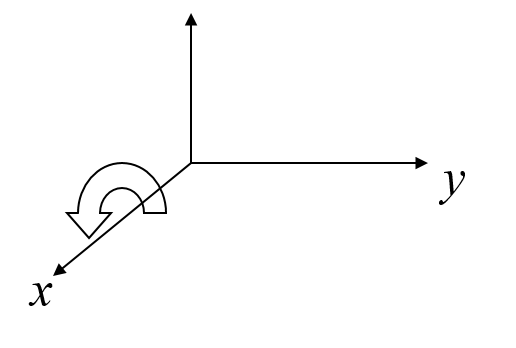
\includegraphics[height=2cm]{geometry/rotate2.png}

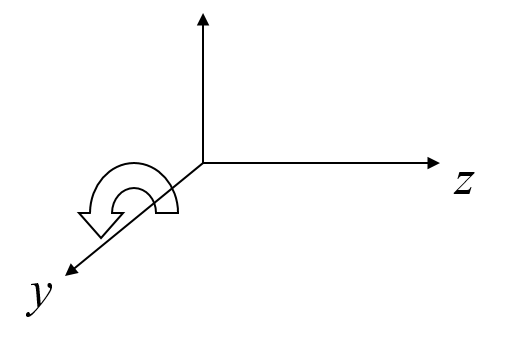
\includegraphics[height=2cm]{geometry/rotate3.png}
\end{multicols}
\end{frame}

\begin{frame}
\frametitle{绕坐标轴旋转}
\framesubtitle{旋转矩阵}
绕z轴:
$(x \ y \ z \ 1)
\left[
    \begin{array}{ c @{\ } c @{\ } c @{\ } c }
        \cos(\gamma)  & \sin(\gamma) & \ \ \ 0 \ \ \ & \ \ \ 0 \ \ \ \\
        -\sin(\gamma) & \cos(\gamma) & \ \ \ 0 \ \ \ & \ \ \ 0 \ \ \ \\
        0             & 0            & \ \ \ 1 \ \ \ & \ \ \ 0 \ \ \ \\
        0             & 0            & \ \ \ 0 \ \ \ & \ \ \ 1 \ \ \
    \end{array}
\right]
=(x' \ y' \ z' \ 1)$

绕x轴:
$(x \ y \ z \ 1)
\left[
    \begin{array}{ c @{\ } c @{\ } c @{\ } c }
       \ \ \ 1 \ \ \ & 0             & 0            & \ \ \ 0 \ \ \ \\
       \ \ \ 0 \ \ \ & \cos(\gamma)  & \sin(\gamma) & \ \ \ 0 \ \ \ \\
       \ \ \ 0 \ \ \ & -\sin(\gamma) & \cos(\gamma) & \ \ \ 0 \ \ \ \\
       \ \ \ 0 \ \ \ & 0             & 0            & \ \ \ 1 \ \ \
    \end{array}
\right]
=(x' \ y' \ z' \ 1)$

绕y轴:
$(x \ y \ z \ 1)
\left[
    \begin{array}{ c @{\ } c @{\ } c @{\ } c }
        \cos(\gamma)  & \ \ \ 0 \ \ \ & -\sin(\gamma) & \ \ \ 0 \ \ \ \\
        0             & \ \ \ 1 \ \ \ & 0             & \ \ \ 0 \ \ \ \\
        \sin(\gamma)  & \ \ \ 0 \ \ \ & \cos(\gamma)  & \ \ \ 0 \ \ \ \\
        0             & \ \ \ 0 \ \ \ & 0             & \ \ \ 1 \ \ \
    \end{array}
\right]
=(x' \ y' \ z' \ 1)$

\end{frame}

\begin{frame}
\frametitle{绕任意直线旋转}
\pause
有了绕坐标轴旋转的方法之后，就可以得到绕任意直线旋转的方法。\newline \newline

\pause
先把该向量变成以(0,0,0)为起点、(a,b,c)为终点，然后把该向量以x轴为旋转轴把向量旋入平面xy，再以y轴为旋转轴把向量旋入平面yz，这样最后的向量就变成了z轴，直接绕z轴旋转即可，旋转完毕之后再旋转回来。\newline \newline

\pause
分五次绕坐标轴旋转操作
\end{frame}

\begin{frame}
\frametitle{绕任意直线旋转}
\framesubtitle{第一步}
\pause
以x轴为旋转轴把向量旋入平面xy

旋转的角度就等于V在平面yz上的投影向量与z轴的夹角

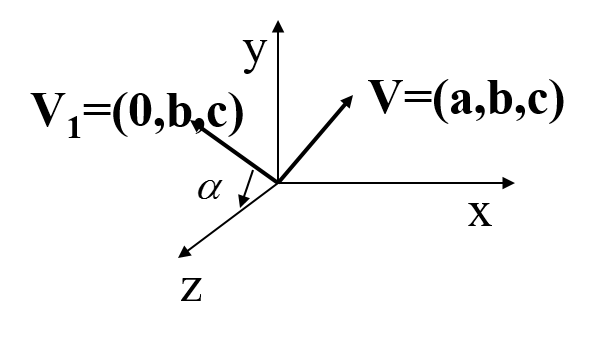
\includegraphics[height=3cm]{geometry/rotate4.png}

$R_x=
\left[
\begin{array}{ c @{\ } c @{\ } c @{\ } c}
    1 & 0                             & 0                            & 0 \\
    0 & \frac{ c }{ \sqrt{b^2+c^2} }  & \frac{ b }{ \sqrt{b^2+c^2} } & 0 \\
    0 & -\frac{ b }{ \sqrt{b^2+c^2} } & \frac{ c }{ \sqrt{b^2+c^2} } & 0 \\
    0 & 0                             & 0                            & 1
\end{array}
\right]
$
\end{frame}

\begin{frame}
\frametitle{第二步}
\pause
以y轴为旋转轴把向量旋入平面yz

V在第一步旋转之后的坐标为$(a,0,\sqrt{b^2+c^2})$,旋转的角度就是现在V与z轴的夹角

\pause
$R_y=
\left[
\begin{array}{ c @{\ } c @{\ } c @{\ } c}
    \frac{ \sqrt{b^2+c^2} }{ \sqrt{a^2+b^2+c^2} } & 0 & \frac{ a }{ \sqrt{a^2+b^2+c^2} }              & 0 \\
    0                                             & 1 & 0                                             & 0 \\
    -\frac{ a }{ \sqrt{a^2+b^2+c^2} }             & 0 & \frac{ \sqrt{b^2+c^2} }{ \sqrt{a^2+b^2+c^2} } & 0 \\
    0                                             & 0 & 0                                             & 1
\end{array}
\right]
$
\end{frame}

\begin{frame}
\frametitle{第三步}
\pause
绕z轴旋转指定的角度$\theta$

$R_z=
\left[
\begin{array}{ c @{\ } c @{\ } c @{\ } c}
    \cos(\theta)  & \sin(\theta) & 0 & 0 \\
    -\sin(\theta) & \cos(\theta) & 0 & 0 \\
    0             & 0            & 1 & 0 \\
    0             & 0            & 0 & 1
\end{array}
\right]
$
\end{frame}

\begin{frame}
\frametitle{第四步}
\pause
把第二步反向还原。即把旋转的角度取相反数，即把sin值取反。

${R'}_y=
\left[
\begin{array}{ c @{\ } c @{\ } c @{\ } c}
    \frac{ \sqrt{b^2+c^2} }{ \sqrt{a^2+b^2+c^2} } & 0 & -\frac{ a }{ \sqrt{a^2+b^2+c^2} }             & 0 \\
    0                                             & 1 & 0                                             & 0 \\
    \frac{ a }{ \sqrt{a^2+b^2+c^2} }              & 0 & \frac{ \sqrt{b^2+c^2} }{ \sqrt{a^2+b^2+c^2} } & 0 \\
    0                                             & 0 & 0                                             & 1
\end{array}
\right]
$
\end{frame}

\begin{frame}
\frametitle{第五步}
\pause
把第一步还原。

${R'}_x=
\left[
\begin{array}{ c @{\ } c @{\ } c @{\ } c}
    1 & 0                            & 0                             & 0 \\
    0 & \frac{ c }{ \sqrt{b^2+c^2} } & -\frac{ b }{ \sqrt{b^2+c^2} } & 0 \\
    0 & \frac{ b }{ \sqrt{b^2+c^2} } & \frac{ c }{ \sqrt{b^2+c^2} }  & 0 \\
    0 & 0                            & 0                             & 1
\end{array}
\right]
$
\end{frame}

\begin{frame}
\frametitle{合并}
\pause
把五个矩阵相乘看起来比较复杂，不过可以强制把向量V模长调整为$\sqrt{a^2+b^2+c^2}=1$

\pause
然后经过一系列复杂的矩阵乘法，可以求出向量旋转的矩阵。

\pause
为了排版方便，令$SIN=\sin(\theta),COS=\cos(\theta)$

$
\left[
\begin{array}{ c @{\ } c @{\ } c @{\ } c}
    a^2+(1-a^2)COS & ab(1-COS)+cSIN & ac(1-COS)-bSIN & 0 \\
    ab(1-COS)-cSIN & b^2(1-COS)+COS & bc(1-COS)+aSIN & 0 \\
    ac(1-COS)+bSIN & bc(1-COS)-aSIN & c^2(1-COS)+COS & 0 \\
    0              & 0              & 0              & 1
\end{array}
\right]
$
\end{frame}

\section{直线}

\subsection{点到直线距离}
\begin{frame}
\pause
三维直线的存储也有两点式和参数式两种。

\pause
求点C到直线AB的距离也类似，$\frac{ \overrightarrow{AB} \times \overrightarrow{AC} } { |AB| }$。

\pause
然后用和二维一样的方法可以求出点到直线的投影。
\end{frame}

\subsection{空中直线距离}
\begin{frame}
\pause
如果两直线有交点，则距离为0。

\pause
如果两直线平行，就相当于是点到直线的距离。

\pause
设两直线的方向向量为$\overrightarrow{a},\overrightarrow{b}$。并且在直线上各任取一点A和B，那么B-A在$\overrightarrow{a} \times \overrightarrow{b}$上的投影的模即为距离。即
\begin{displaymath}
    d=\left| \frac{ (\overrightarrow{a} \times \overrightarrow{b}) \cdot (B-A) }{ |\overrightarrow{a} \times \overrightarrow{b}| } \right|
\end{displaymath}
\end{frame}

\subsection{三维直线求交}
\begin{frame}
\pause
三维直线求交有两种方法。

\pause
第一种是利用与二维直线求交一样的思路，利用叉积算面积并计算。但是这里有一个关键问题：三维叉积求出的是一个向量，向量的模长才是面积，但是求向量的模长需要用到开方操作，这样就丢失了面积的正负。所以我们可以暴力枚举面积正负求出交点再判断是否在直线上。

\pause
第二种是投影法，我们先求出两条直线投影到平面z=0的交点，然后再判断z值是否满足要求。但是这里会遇到特殊情况:$dx=0$或$dy=0$，这时我们需要切换投影面，我们可以把$z=0,y=0,x=0$这三个投影面都尝试一遍，如果都不行则两直线重合或平行，否则就可以找到交点。
\end{frame}

\subsection{异面直线公垂线}
\begin{frame}
\label{hehe}
\pause
求异面直线AB和CD的公垂线PQ。

PQ要同时垂直于AB和CD，则会垂直于AB和CD所在平面，所以就垂直于$\overrightarrow{AB} \times \overrightarrow{CD}$

则$| \overrightarrow{PQ} |=\frac{| \overrightarrow{n} \times \overrightarrow{AC} |}{| \overrightarrow{n} |}$
\end{frame}

\subsection{空中线段距离}
\begin{frame}
\frametitle{求空中线段AB和CD的距离}
\pause
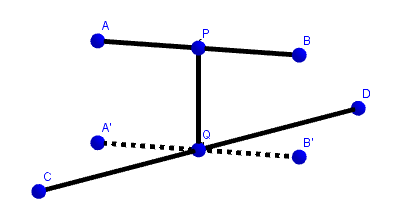
\includegraphics[height=2cm]{geometry/3dline.png}

方法分三步:
\begin{enumerate}
    \item 求出两条线段所在直线的公垂线PQ
    \item 将两个直线投影到与公垂线垂直的平面，计算平面内两条线段的距离dis
    \item $ans=\sqrt{(|PQ|^2+dis^2)}$
\end{enumerate}
令$\overrightarrow{n}=\overrightarrow{AB} \times \overrightarrow{CD}$

公垂线可以用叉积求得。见\textcolor{purple}{\ref{hehe}}

$A'=A+|\overrightarrow{PQ}| \frac{\overrightarrow{n}}{|\overrightarrow{n}|},B'=B+|\overrightarrow{PQ}| \frac{\overrightarrow{n}}{|\overrightarrow{n}|}$
\end{frame}

\section{平面}

\subsection{三维平面表示}
\begin{frame}
\pause
三维平面可以用方程列出一般式，但是一般比较麻烦。

\pause
比较常用的是点法式，用平面上的一个点P和与这个平面垂直的法向量$\overrightarrow{v}$来描述。
\end{frame}

\subsection{点到平面距离}
\begin{frame}
\pause
点A到平面$(P,\overrightarrow{v})$的距离，就是$\overrightarrow{AP}$，在v上的投影长度。
\begin{displaymath}
    \frac{ \overrightarrow{AP} \times \overrightarrow{v} }{ |\overrightarrow{v}| }
\end{displaymath}
\end{frame}

\subsection{点到平面投影}
\begin{frame}
\pause
知道了点到平面的距离，利用法向量就可以求出点到平面的投影。

\pause
有时一些几何对象在同一个平面上，我们希望给予平面上每一个点一个二维坐标，从而把问题转化为一个二维问题解决。

\pause
我们需要在平面上指定一个点O为源点，以及一个向量$\overrightarrow{x}$作为横轴，一个向量$\overrightarrow{y}$作为纵轴，要求$\overrightarrow{x} \bot \overrightarrow{y}$。

对于每一个点A，在当前坐标系下其横坐标为$A-O$在x上的投影长度$\frac{ (A-O) \times \overrightarrow{x} }{ |\overrightarrow{x}| }$，纵坐标亦然。

\pause
为了方便，我们可以把$| \overrightarrow{x} |$和$| \overrightarrow{y} |$缩放为1。

若已知平面上一点以此坐标系投影的坐标为$(a,b)$，则还原到三维坐标为$O+a\overrightarrow{x}+b\overrightarrow{y}$
\end{frame}

\subsection{直线和面交点}
\begin{frame}
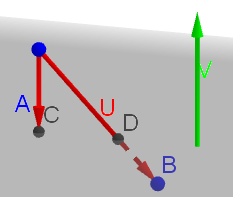
\includegraphics[height=3cm]{geometry/3dgraph.png}

求直线AB和平面$(C,\overrightarrow{v})$的交点。

首先求出A到平面C的垂直向量$\overrightarrow{AC}$

如果$\overrightarrow{AB} \perp \overrightarrow{AC}$则线面平行，无解。

否则我们需要找到的点D满足$\overrightarrow{AD}$在$\overrightarrow{AC}$上的投影恰好为$\overrightarrow{AC}$。即$\overrightarrow{AD} \times \overrightarrow{AC}=|AC|^2$

同时$\overrightarrow{AD}:\overrightarrow{AB}=| \overrightarrow{AD} \times \overrightarrow{AC} |:|\overrightarrow{AB} \times \overrightarrow{AC} |$

所以$\overrightarrow{AD}=\overrightarrow{AB}
\frac{ | \overrightarrow{AD} \times \overrightarrow{AC} |}{|\overrightarrow{AB} \times \overrightarrow{AC} |}
=\overrightarrow{AB} \frac{|AC|^2}{| \overrightarrow{AB} \times \overrightarrow{AC} |}$

\end{frame}

\subsection{面和面的交线}
\begin{frame}
设两平面的法向量为$h_1,h_2$。

若它们平行，则两平面平行或重合。

否则，交线的方向向量与$h_1,h_2$垂直，即为$h_1 \times h_2$，那么就只需求出交线上的一点即可。

可以随机生成一条在第一平面内，但不与第二平面平行的直线，求它与第二平面的交点。
\end{frame}

\subsection{二面角}
\begin{frame}
\pause
就是两个平面法向量的夹角。
\end{frame}

\section{球}
\subsection{球与直线的交点}
\begin{frame}
\pause
首先求球心到直线的距离h和垂足。

\pause
若$h>r$则无解。

\pause
两个交点到垂足的距离为$\sqrt{r^2-h^2}$，缩放直线向量求得即可。
\end{frame}

\subsection{球与平面或球的交圆}
\begin{frame}
\pause
先求交圆的圆心，再求出半径。因为是三维空间，所以还要表面圆所在的平面。
\end{frame}

\section{三维凸包}

\subsection{定义}
\begin{frame}
\pause
同二维凸包一样定义：如果点集中存在点A,B，则线段AB上的所有点都必须在凸包内

\pause
不过还要加上一条：凸包的每一个面都满足，所有点只会分布在面的一侧。

\pause
在满足这两个条件的情况下，取体积最小的多面体。

\pause
结论：三维凸包的边数是线性的

\pause
证明：我们可以把三维凸包的表面展开成一个平面图。由欧拉公式，F(面数)+V(点数)-E(边数)=2

一条边恰归属于两个面，一个面有$\ge 3$条边，$2E \ge 3F$。

可得$E \le 3V-6,F \le 2V-4$
\end{frame}

\subsection{构造}

\begin{frame}
\frametitle{方法一}
\framesubtitle{暴力法}
\pause
可以很自然地想到一种暴力：

\pause
$O(n^3)$枚举每一个面，然后$O(n)$check一下每一个点是否都在面内。
\end{frame}

\begin{frame}
\frametitle{方法二}
\framesubtitle{增量法}
\pause
先取出点集中的4个点，这4个点组成的四面体为初始凸包。(要求这4个点构成的凸包体积不为0)

然后添加其他各点。如果这个点在已知凸包内部，则直接跳过。否则，找出可视部分与不可视部分的分界线，删去所有的可视面，然后将所有分界线上的边与该点构成的面作为新凸包的面。

\begin{multicols}{2}
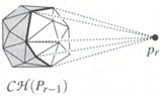
\includegraphics[height=2cm]{geometry/3dtubao.png}

黑色的边被称为地平线。地平线的两端，一定是一个可见面一个不可见面。

然后删除可见面，用新点连接地平线的每一条边。
\end{multicols}

\pause
要注意的是一个面上的点的顺序，两个不同的顺序代表的是两个不同的半空间。
\pause
复杂度$O(n^2)$。同时这个方法是在线的。
\end{frame}

\begin{frame}
\frametitle{方法三}
\framesubtitle{卷包裹法}
\pause
卷包裹法就是一张纸紧贴着凸包的一条边AB沿AB的右手边收拢，直到遇到顶点C为止

那么ABC是凸包上的一个面

递归：沿$AC$和$CB$方向搜索

\pause
初始时找到一条一定在凸包中的边$AB$，然后调用函数$wrap(\overrightarrow{AB})$

\pause
复杂度$O(nh)$
\end{frame}

\begin{frame}
\frametitle{方法四}
\framesubtitle{随机增量法}
\pause
方法二的增量复杂度瓶颈在于每次都要扫描所有凸包上的边来找到可见面与不可见面的边界。

考虑增量算法的一个改进，寻找地平线时不枚举所有面，而是利用之前的信息

\pause
定义二分图$C=(P,F,E)$，如果一个点P看得到一个面F，在他们之间连边，得到的二分图称为冲突图(conflict graph)

冲突图的两部分别是未处理的点和已存在的面
\end{frame}

\begin{frame}
\frametitle{方法四}
\framesubtitle{随机增量法}
\pause
\begin{multicols}{2}
查询可见面:

直接从冲突图里面读取

设置点为已处理，删除平面:

直接对二分图进行操作

加入新面:

枚举每个点，判断可见性

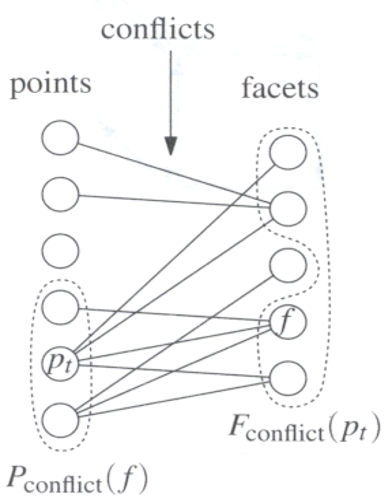
\includegraphics[height=5cm,width=4cm]{geometry/3dtubao2.png}
\end{multicols}

但是加入新面时还是要扫一遍所有的点，复杂度仍然是平方。
\end{frame}

\begin{frame}
\frametitle{方法四}
\framesubtitle{随机增量法}
\pause
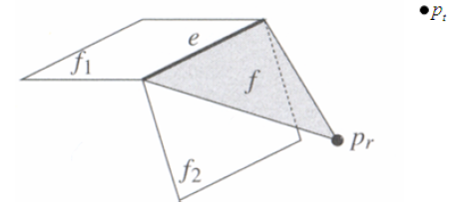
\includegraphics[height=3cm]{geometry/3dtubao3.png}

新的面一定连接当前处理点Pr和一条地平线e

假设e原先连接两个面f1,f2（恰好有一个面将被剔除）

证明：点Pt若能看见f，必定能看见f1或f2

在加入facet时只需要考虑能见到f1/f2的点

\pause
据说复杂度是$nlogn$的，但是并不会证明。不过实际复杂度确实非常优秀。
\end{frame}

\begin{frame}
\frametitle{方法五}
\framesubtitle{分治法}
\pause
和2维一样的思路，分块构造凸包，然后进行合并。 \newline \newline

\pause
鉴于三维凸包的合并非常复杂，并且很容易把复杂度写挂，所以仅供了解。
\end{frame}

\begin{frame}
\frametitle{方法六}
\framesubtitle{QuickHull}
\pause
把二维的情况稍稍拓展就可以做三维了。

调用函数$Quickhull(P_0,P_1,P_2)$

找到离平面$(P_0,P_1,P_2)$最远的点K

递归:

$Quickhull(K,P_0,P_1)$

$Quickhull(K,P_1,P_2)$

$Quickhull(K,P_2,P_0)$ \newline \newline

\pause
同样，Quickhull算法被经常运用在三维乘积问题中。(如三维最小乘积生成树)
\end{frame}

\subsection{三维凸包的体积、重心}
\begin{frame}
\frametitle{重心}
\pause
几何定义：顶点和对面重心的连线交点为重心。
$G=\frac{A+B+C+D}{4}$

\pause
可以推广到N维单纯形上

\pause
多面体重心：

以原点进行三角剖分

\begin{displaymath}
G=\frac{\sum V_iG_i}{\sum V_i}
\end{displaymath}

假设各个面是$i \rightarrow j \rightarrow k$

\begin{displaymath}
G_i=\frac{P_i+P_j+P_k}{4},V_i=\frac{(P_i \times P_j) \cdot P_k}{6}
\end{displaymath}

\begin{displaymath}
G= \sum_i \frac{(P_i+P_j+P_k)*((P_i \times P_j) \cdot P_k)}{24V}
\end{displaymath}
\end{frame}

\subsection{三维半空间交}
\begin{frame}
\textcolor{red}{\huge{我不会。。。QAQ}}
\end{frame}


\part{4}
\begin{frame}{Part4}{exercise}
\textcolor{purple}{\huge{下面进入杂题选讲}}
\end{frame}

\section{水题合集}

\begin{frame}
\pause
\begin{description}[<+->]
    \item[POJ1066] 线段相交
    \item[POJ1654] 多边形求面积
    \item[POJ1127] 线段相交+并查集
    \item[POJ2318] 点在凸多边形内，推荐入门
    \item[POJ2653] 线段相交，推荐入门
    \item[POJ1410] 线段与矩形相交
    \item[POJ1269] 直线与直线关系判断，求交点，推荐入门
    \item[POJ3304] 直线与线段相交
\end{description}
\end{frame}

\section{杂题}

\begin{frame}
\frametitle{CF744D Hongcow Draws a Circle}
\pause
平面上有n个红点和m个蓝点$(1 \le n,m \le 1000)$。

你要找一个半径最大的圆，使得它包含至少一个红点，并且不包任何一个蓝点。

如果答案可以无限大输出-1。

\pause
如何判-1？只要所有蓝点构成的凸包没有包含(不能在边界上)所有红点则无解。

\pause
如果有解，那么最大的圆上一定有一个蓝点(否则可以继续把圆扩大)
\end{frame}

\begin{frame}
\frametitle{CF744D Hongcow Draws a Circle}
\framesubtitle{方法一}
\pause
二分答案mid，然后枚举所有的蓝点k。

对每一个点都画一个半径为mid的圆。

如果某个圆和k有交，那么在交的哪一段极角区域打上标记。

然后做一遍扫描线，判断是否存在某个极角区域只有红标记没有蓝标记。

\textbf{pay \ atttention:}直接二分答案是不满足单调性的，因为把半径加长可能导致与蓝点相交，把半径缩短可能导致无法连接到红点。所以我们需要找到能连接到红点的最短距离。那么我们先对所有的红点为中心做一次二分答案，求出红点在圆上时半径最大值。然后再以蓝点为中心进行二分答案，以红点得到的答案为下界，这样答案就是满足单调性的了。
\end{frame}

\begin{frame}
\frametitle{CF744D Hongcow Draws a Circle}
\framesubtitle{方法二}
\pause
枚举了蓝点k之后，我们要找一个经过点k，包含至少一个红点，且不能包含蓝点的圆。

考虑反演，过k点的圆反演之后变成了一条直线，圆内的点就是直线外侧的点。

圆的半径和直线到k的距离成反比，所以我们需要最小化直线到k的距离。

\pause
分析一下可以发现，最优直线一定是蓝点构成的凸包上的边。

那么我们枚举完k之后构出反演之后的凸包，然后枚举凸包上所有边，再$O(n)$判断一下这条直线外侧是否有红点。

看起来复杂度是$nm^2$的，但是我们可以构出原图中蓝点的三角剖分。对于点k而言，只有在三角剖分中与点k有边的点才会出现在反演后的图的凸包中。所以复杂度是$n*$三角剖分边数总和的。注意到三角剖分是一个平面图，所以边数是线性的。
\end{frame}

\begin{frame}
\frametitle{清华集训2016 定向越野}
\pause
平面上有n个圆，互相之间不相交。

要从平面上一个点到达另一个点，不能经过任何圆盘内部。求最短路。

$n \le 500$

\end{frame}

\begin{frame}
\frametitle{清华集训2016 定向越野}
\pause
最终路径一定是若干条圆与圆之间的公切线和若干段圆周连接而成。

\pause
求与其他圆不相交公切线，构图。

\pause
求最短路(根据题目特性对于每个圆做特殊处理)。

\pause
可以暴力构图，$O(n^2)$枚举所有公切线，$O(n)$检验一条公切线是否穿过了其它圆。

\pause
可以用扫描线优化到$O(n^2logn)$
\end{frame}

\begin{frame}
\pause
给定平面上的n个点，求它们的欧几里得最小生成树

$n \le 10^5$

\pause
构出三角剖分，做最小生成树。
\end{frame}

\begin{frame}
\frametitle{CF536 C Tavas and Pashmaks}
\pause
题目大意:$n$个人比赛，要游泳$Sm$，跑步$Rm$(S,R未知),已知每个人的$V_s,V_r$,求所有可能取胜的人

\pause
我们把一个人看成平面上一个点$(\frac{1}{V_s},\frac{1}{V_r})$。那么一个人花费的时间就是与$(S,R)$的点积。

很显然，点集中与某个向量点积最大的点一定位于凸包上。

我们构出凸包，然后输出从横坐标最小的点到纵坐标最小的点这一段。
\end{frame}

\begin{frame}
\frametitle{cyclotron}
\pause
给你N个不经过原点的圆。让你求一个过原点的圆，使得与它有交点的圆尽量多。（所求的圆可以退化为直线）$N \le 1000$

\pause
以原点为中心反演，那么现在问题变成了：求一条直线使得与它有交点的圆尽量多。

\pause
很显然答案一定可以与两个圆相切(否则可以把直线进行偏转)

枚举一个圆，然后求出其它圆和这个圆相切对应的极角范围，然后扫描线即可。
\end{frame}

\begin{frame}
\frametitle{Codechef QPOINT}
\pause
在二维平面内，给定n个没有公共点的简单多边形。每次询问一个点，回答这个点属于哪个简单多边形，强制在线。

$n \le 10^5$，简单多边形的顶点数之和$\le 3*10^5$，询问个数$\le 10^5$。

\pause
裸题。

先特判在一条竖线上的情况，其余的直接做可持久化扫描线。
\end{frame}

\begin{frame}
\frametitle{圆的面积并}
\pause
求n个圆的并的面积$(n \le 1000)$

\pause
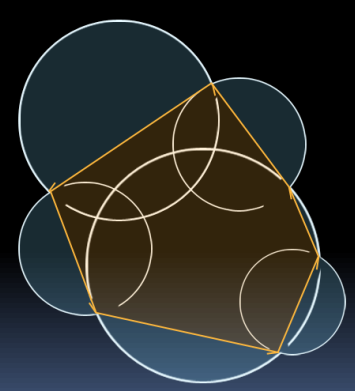
\includegraphics[height=4cm]{geometry/bing.png}

如图，最后形成的图形是由很多弓形和多边形组成的。

弓形的面积可以单独计算，多边形的面积可以用叉积算。
\end{frame}

\begin{frame}
\frametitle{圆的面积并}
\pause
如图，对于每个圆，用其它的圆与之求交，找到所有没有被覆盖的圆弧。圆弧须以逆时针序表示。

对于每条圆弧，累加其弓形的面积，以及这条边的有向面积。

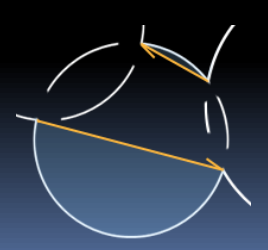
\includegraphics[height=5cm]{geometry/bing2.png}
\end{frame}

\begin{frame}
\frametitle{圆的面积并}
\framesubtitle{有洞？}
\pause
由于我们用的是叉积-有向面积，所以洞会被自动抵消。

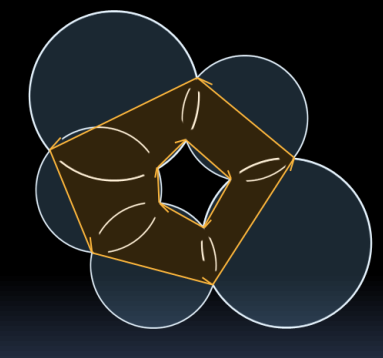
\includegraphics[height=6cm]{geometry/bing6.png}
\end{frame}

\begin{frame}
\frametitle{最小圆}
\pause
求解包含某个点集的半径最小的圆

\pause
很显然，最终的圆一定会被边界点卡住而无法向任何方向平移。

\pause
要卡住一个圆，要么是一对点$(a,b)$，满足圆心在直线AB上，要么是三个不相同的点$(a,b,c)$。

\pause
所以我们枚举点a，如果存在点b到a的距离大于当前答案则把圆心设为ab中点，半径为$\frac{|ab|}{2}$，再枚举点c,如果c到圆心的距离大于$\frac{|ab|}{2}$则把圆心切换为abc的中点。
\end{frame}

\begin{frame}
\frametitle{判断两个多边形的交面积是否$>0$}
\pause
Case \ 1:有两条线段严格相交(一条线段上的点不允许在另一条直线上)

直接叉积判断即可

\pause
Case \ 2:有一个点在另一条线段上。

判断这个点相邻的两个点是否分布两侧

\pause
Case \ 3:有两个点相同

判断这两个点相邻一共四个点的位置关系。
\end{frame}

\begin{frame}
\frametitle{POJ3675}
\pause
求多边形和圆的交

\pause
看起来非常复杂，但是我们可以把多边形拆成若干个三角形分别计算。

利用叉积的方向，我们可以取任意点为基准点，自然取圆心最方便计算。

\pause
现在的任务就是计算一个以原点为圆心，半径为R的圆和$\triangle ABC$的交面积。
\end{frame}

\begin{frame}
\frametitle{POJ3675}
\framesubtitle{Case 1}
\pause
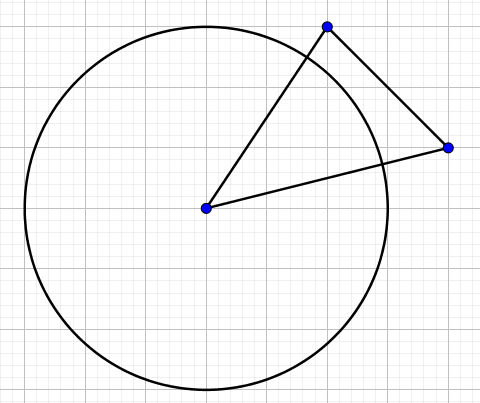
\includegraphics[height=5cm]{geometry/case1.png}

线段AB完全在圆外

面积就是一段扇形的面积。
\end{frame}

\begin{frame}
\frametitle{POJ3675}
\framesubtitle{Case 2}
\pause
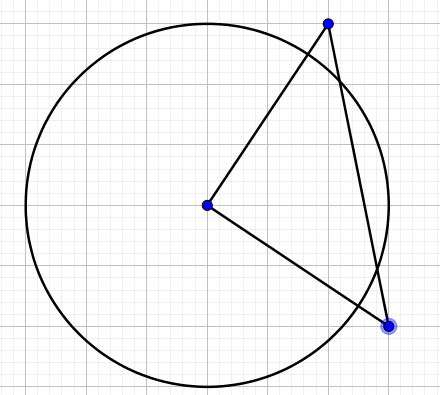
\includegraphics[height=5cm]{geometry/case2.png}

点AB完全在圆外，但是线段AB与圆有交

\pause
两段扇形+一个三角形
\end{frame}

\begin{frame}
\frametitle{POJ3675}
\framesubtitle{Case 3}
\pause
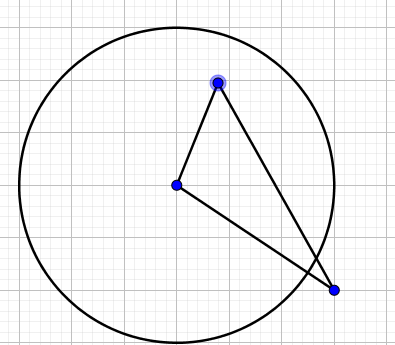
\includegraphics[height=5cm]{geometry/case3.png}

AB一个在圆外一个在圆内

\pause
一个扇形+一个三角形
\end{frame}

\begin{frame}
\frametitle{POJ3675}
\framesubtitle{Case 4}
\pause
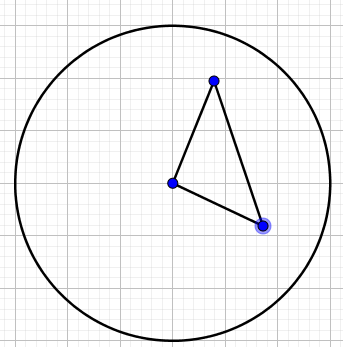
\includegraphics[height=5cm]{geometry/case4.png}

AB都在圆内

\pause
面积就是$S_{\triangle}ABC$
\end{frame}

\begin{frame}
\frametitle{清华集训2012Day4T3 阳光}
\framesubtitle{题目描述}
\pause
为了督促同学们长跑，体育组制作了“阳光长跑卡”，并要求同学们通过刷卡来证明自己跑过的距离。为了防止同学抄近路，体育组又在跑到上设置了很多个刷卡点，要求同学们依次刷过。为了防止同学互相代替刷卡，体育组便安排了一个老师在现场监督。然而，老师的视野范围有限，可能无法监督到所有的刷卡点。为了解决这一问题，体育组的老师来向你寻求帮助。

简要地说，我们可以把跑道看做一个以原点为圆心、半径为r的圆。监督的老师站在原点处，视野范围为一个给定的n边形，且顶点顺序满足以原点为中心的极角序。现让你在跑到上放置m个等距的刷卡点，使得尽可能多的刷卡点落在老师的视野范围内(视野范围包含多边形边界)。
\end{frame}

\begin{frame}
\frametitle{清华集训2012Day4T3 阳光}
\framesubtitle{sol}
\pause
首先求出圆上哪些区域被多边形覆盖，可以用$O(n)$段极角区间来表示。\newline \newline

\pause
我们的任务是确定一个量$d \in [0,\frac{2 \pi}{m})$，然后把把所有的刷卡点放在$k*\frac{2 \pi}{m}+d$上。\newline \newline

\pause
用点事件可以做到$nlogn$
\end{frame}

\begin{frame}
\frametitle{world final 2017 Airport Construction}
\pause
给你一个$n$个点的多边形，求它的直径。

\pause
例:
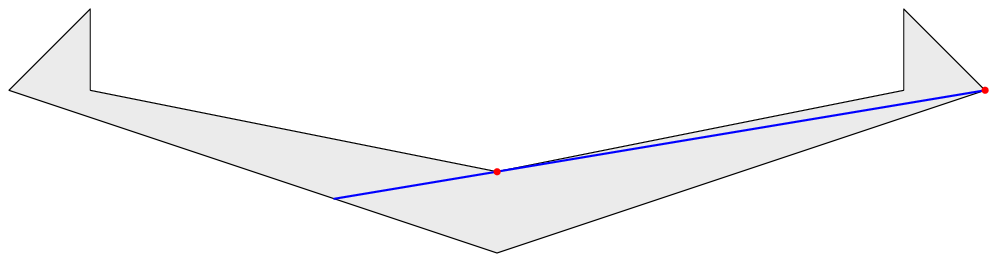
\includegraphics[height=3cm]{geometry/wf.png}

\pause
$n \le 200$

\pause
容易分析得出，直径一定至少经过其中两个点。否则可以调整变得更优。

可以先$n^2$枚举所有直线，然后判断在多边形内的最大线段长度。(难点)
\end{frame}

\begin{frame}
\frametitle{world final 2017 Airport Construction}
\framesubtitle{sol}
\pause
但是有很多种情况，稍微不注意可能就会挂。

\pause
\begin{multicols}{3}
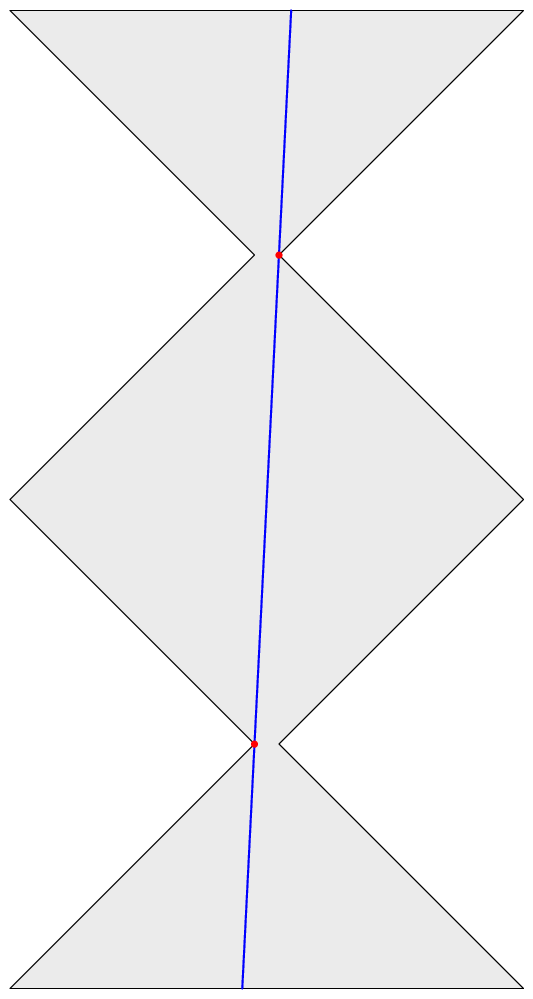
\includegraphics[width=3.5cm,height=3cm]{geometry/wf2.png}
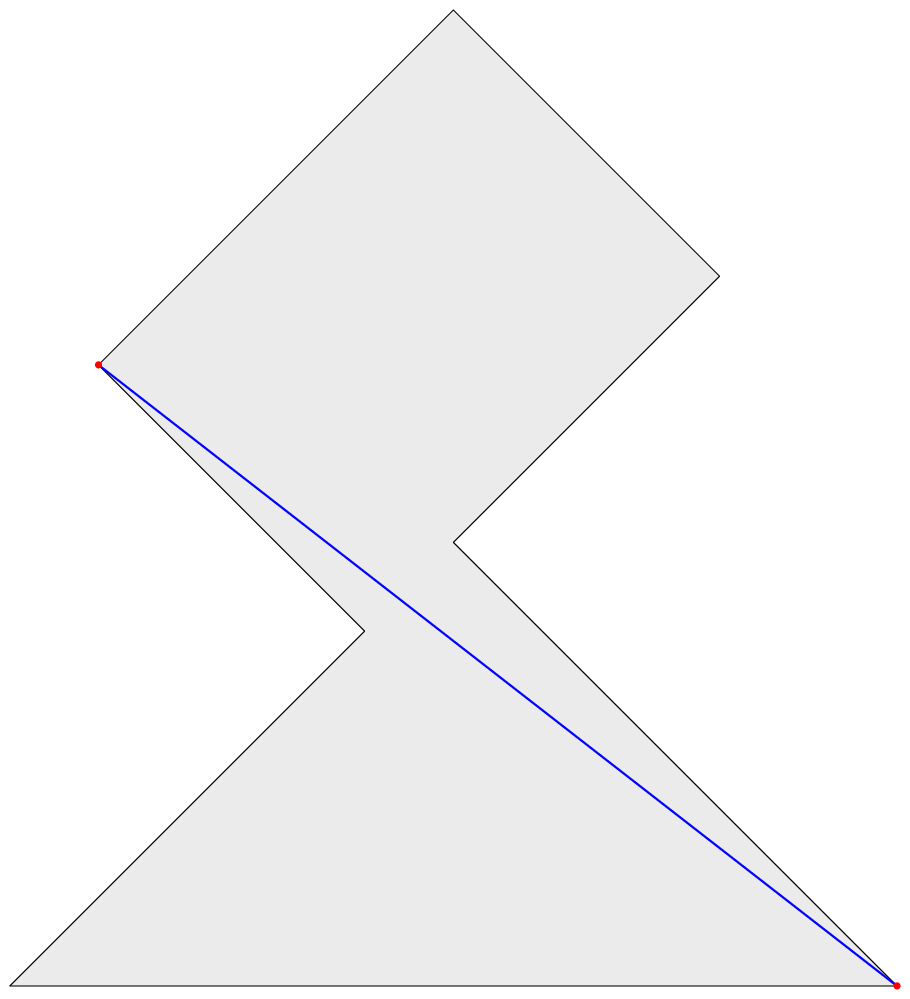
\includegraphics[width=3.5cm,height=3cm]{geometry/wf3.png}
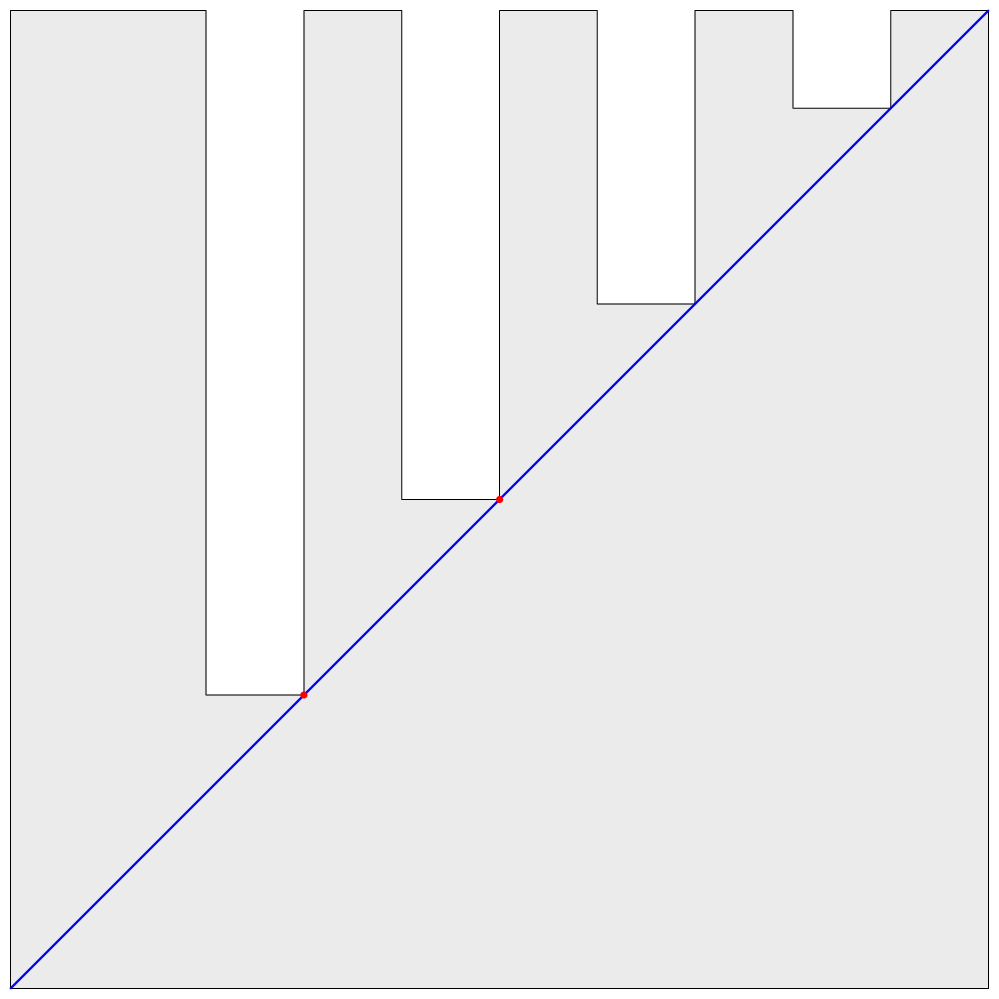
\includegraphics[width=4cm,height=3cm]{geometry/wf4.png}
\end{multicols}

\pause
而且还要特别注意的是：有可能枚举的直线都在多边形外。

这里推荐一种好写的方法：把直线和多边形的所有交点都记录到数组$cross[1 \cdots m]$中并排序，然后$cross[2k-1] \rightarrow cross[2k]$就是所有在多边形内部的区间。
\end{frame}

\begin{frame}
\frametitle{CTSC2017 投影}
\pause
k维空间中有n个黑点与n个白点。我们为每一个黑点确定一个互不相同的对应的白点，这样一共有$n!$种对应方法。我们定义这n个黑点与n个白点之间的“移动距离”为，在所有的对应方法中，对应的黑点与白点之间的 n个\textbf{欧几里德}距离的和的\textbf{最小值}。

你得到了三维空间中的n个黑点与n个白点。你想把它们投影到一个$k(1 \le k \le 2)$维子空间上。一维子空间就是三维空间中的一条直线，二维子空间则是三维空间中的一个平面。一个点在一个子空间中的投影点就是这个子空间中距离它最近的点。例如，$(0,0,0),(1,1,0),(1,0,0),(0,1,0)$这四个点投影到$x-y=0,z=0$这条直线上之后，得到的投影点是$(0,0,0),(1,1,0),(0.5,0.5,0),(0.5,0.5,0)$。

求着n个黑点和n个白点投影到k维子空间之后移动距离最大值。
\end{frame}

\begin{frame}
\frametitle{CTSC2017 投影}
\framesubtitle{30分：二维投影一维}
\pause
如果已知投影直线，求答案是非常轻松的。

按照在直线上的投影坐标排序，按照顺序匹配一定保证最优。(这个很好理解，交叉匹配不可能使答案更优)

\pause
如果在某段极角范围内，点在直线上的投影坐标相对顺序不变，则我们可以列出移动距离关于极角的函数，然后求得最值。

如果$A,B$投影坐标相对顺序发生变化，则发生变化的时刻为投影直线垂直于直线$AB$。

发生变化的事件个数为$O(n^2)$，扫描线找到所有区间，对这$O(n^2)$个区间分别求解。

\pause
现在的关键问题是，如果找到最优极值点。
\end{frame}

\begin{frame}
\frametitle{CTSC2017 投影}
\framesubtitle{30分：二维投影一维}
\pause
我在考场上想出一个做法，如果直线的极角为$\alpha$，一组匹配点的极角为$\beta$，欧几里得距离为d，则他们在直线上投影距离为$d \cos(\alpha-\beta)$

用三角函数公式，可以把所有匹配点的投影距离之和表示成$a\sin(\alpha)+b\cos(\alpha)$的形式。通过辅助角公式我们知道，这个函数可以通过一个三角函数的平移、拉伸得到，所以满足在跨度不超过$\pi$的一段区间，该函数为单峰函数，可以用三分法求得极值。\pause 复杂度为$O(n^2 \log n)$。\newline \newline

\pause
然而遗憾的是，$\cos$函数应该取绝对值，否则如果极角差$> \frac{\pi}{2}$则会爆负数。。。QAQ，然后我就愉快地爆零了。
\end{frame}

\begin{frame}
\frametitle{CTSC2017 投影}
\framesubtitle{30分：二维投影一维}
\pause
所以还要加上改动：对于一组匹配点$(a,b)$，在极角转过$\frac{\pi}{2}$之后要切换三角函数的符号。

每次修改函数值时，都要根据当前极角区间调整三角函数的符号。

\pause
std用了更优的方法。

对于所有的匹配$(a_i,b_i)$，我们统计出$(X,Y)=\sum_{i=1}^{n} (x_{b_i}-x_{a_i},y_{b_i}-y_{a_i})$

然后移动距离为$(X,Y)$在极角方向上的投影。那么显然极角方向离$(X,Y)$越近越好，根据左右边界范围可以$O(1)$求出最优解。

复杂度$n^2\log n$，不过这里的$\log$仅仅是排序，所以比我的方法快多了。

\pause
这个方法也要注意，当极角转过$\frac{\pi}{2}$后要切换为相反向量。
\end{frame}

\begin{frame}
\frametitle{CTSC2017 投影}
\framesubtitle{100分}
\pause
std的代码太繁杂了，这里就不多介绍。

\pause
xmk的做法是比较值得提倡的。

他用的是模拟退火算法，一开始随机一些平面法向量，然后求出在这些法向量下的移动距离。然后每次以一定概率接受附近的点。

如何求移动距离呢？投影到一维显然排序即可。投影到二维可以暴力一点使用二分图最大权匹配(KM \ or \ 费用流)。
\end{frame}

\begin{frame}{CF35E}
    给定$N$个下边界紧贴$X$轴，上边界在$X$轴上方的矩形 (矩形的四边都平行于坐标轴) 。
    
    求这个矩形的“轮廓”，即输出矩形的并的顶点坐标，要求轮廓相邻的边垂直。

    $N \le 10^5$
\end{frame}

\begin{frame}{CF35E}
    直观上来看，我们每次沿这边界行走，就能得到最后的答案，但是这样处理起来比较复杂。
    
    用另外一种更为简单的思路，我们将最后轮廓中所有的横向线段找出来，再把他们连接起来即可。
    
    考虑某个横坐标所对应的轮廓的纵坐标，实际上是覆盖它的所有横向线段中最高的那条。
    
    我们将所有的端点离散出来(因为转折点的横坐标只会在端点处产生) ，然后按横坐标从小到大依次扫描每个端点，同时维护当前的轮廓的纵坐标
    
    如果纵坐标发生了变化，则我们需要”拐弯”，将这个转折点记录下来即可。
    
    维护当前轮廓的纵坐标可以用系统堆。复杂度$O(n \log n)$。
    
\end{frame}

\begin{frame}{CF67E}

    给定一个简单多边形，第一条边一定平行于坐标轴，问第一条边上有多少个整点可以看到多边形上所有的顶点
    
    (看到的定义为连线段不会落在多边形外部)。

    数据范围: $n \le 1000,x_i,y_i \le 10^6$

    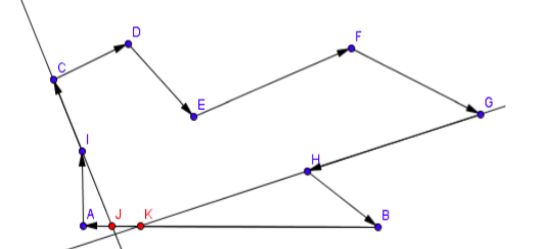
\includegraphics[width=10cm]{geometry/pG1.png}
\end{frame}

\begin{frame}
    我们规定以顺时针遍历所有的边，对于某条边$(a,b)$，它所在的直线的左边的点一定不能同时看到点$a$和$b$。
    
    所以通过这个我们可以在第一条边上加一个限制: 即只有在$(a,b)$所在直线的右边的点才是合法。最后我们对所有的限制取一个交即可。复杂度$O(n\log n)$。
\end{frame}

\begin{frame}
    给定一个凸多边形的三角剖分，从多边形的一个三角形出发，每次可以从一个三角形到其相邻的三角形，但是不能经过重复的三角形。
    
    问哪一对三角形之间的距离最长？

    $N \le 200000$
\end{frame}

\begin{frame}
    平面图的对偶图
    
    这是一棵树！
    
    树的最长链

\end{frame}

\begin{frame}
    给定平面上$n$个圆，问用$k$条线最多能将这$n$个圆分成多少份？

    $N \le 10^3, k \le 10^5$

\end{frame}

\begin{frame}
    若只有一个圆：$1 + K \times (K+1)/2$
    
    若有一条线穿过所有的圆：$1+K \times (K+1)/2+(N-1) \times (K+1)$
    
    希望找到一根线穿过的圆尽可能多
\end{frame}

\begin{frame}
    枚举这条线相切的一个圆（为什么相切？），

    我们可以用角度$[0,2 \pi]$来表示这条直线

    对于每个其它的圆，将会覆盖$[0,2 \pi]$中间的一段区间，然后查询被区间覆盖次数最多是多少次。$O(n\log n)$

\end{frame}

\begin{frame}
\frametitle{CF853E Lada Malina}
\pause
一辆汽车有k个引擎，每个引擎i有一个速度向量$(x_i,y_i)$。现在你可以给每个引擎一个\textbf{实数}参数$v_i \in [-1,1]$，那么汽车最终的速度向量为$(\sum v_ix_i,\sum v_iy_i)$

有n个工厂，i号工厂位于地点$fx_i,fy_i$，厂内有$a_i$辆汽车。

有q个展览会，每个展览会i会在地点$px_i,py_i$举行。每个工厂可以发车前往展览会。展览会$i$还有一个时间限制$t_i$表示汽车需要在$t_i$个单位时间内到达展览会。

求每个展览会最多可以有多少辆汽车在规定时间到达。

$2 \le k \le 10 \ \ 1 \le n,q \le 10^5 \ \ |vx_i|,|vy_i| \in [-1000,1000] \ \ |fx_i|,|fy_i|,|px_i|,|py_i| \le 10^9$
\end{frame}

\begin{frame}
    做法：由于$v_{i}$与$-v_{i}$等价，我们先把每个向量的横坐标变成非负（在此基础上尽量使纵坐标也非负）
    
    把询问变成$p-t\sum v_{j}+\sum w_{j}v_{j}(0 \le w_j \le 2t)$，令$P=p-t\sum v_{j}$
    
    合法的$f_{i}$会在这样一个凸多边形内：从$P$点开始，按斜率从小到大的顺序依次把向量接起来得到一个下凸壳
    
    再从$P$点开始，按斜率从大到小顺序再接出一个上凸壳
    
    想计算这个凸多边形内的点权和，我们只要知道每条边下方（以两个端点向下竖直画射线与这条边围成的区域）的点权和，上凸壳减下凸壳就是答案。
    
    由于斜率只有$k$种，我们每种斜率都做一遍，算出所有同斜率的边以及所有点在这个斜率下的截距，按这个截距的大小顺序，按横坐标建线段树即可统计。
    
    时间复杂度$O(k(n+q)logn)$。
\end{frame}


\end{document}
